%% Modified for NDSS 2020 by DB on 2019/05/15
%%
%% bare_conf.tex
%% V1.3
%% 2007/01/11
%% by Michael Shell
%% See:
%% http://www.michaelshell.org/
%% for current contact information.
%%
%% This is a skeleton file demonstrating the use of IEEEtran.cls
%% (requires IEEEtran.cls version 1.7 or later) with an IEEE conference paper.
%%
%% Support sites:
%% http://www.michaelshell.org/tex/ieeetran/
%% http://www.ctan.org/tex-archive/macros/latex/contrib/IEEEtran/
%% and
%% http://www.ieee.org/

%%*************************************************************************
%% Legal Notice:
%% This code is offered as-is without any warranty either expressed or
%% implied; without even the implied warranty of MERCHANTABILITY or
%% FITNESS FOR A PARTICULAR PURPOSE! 
%% User assumes all risk.
%% In no event shall IEEE or any contributor to this code be liable for
%% any damages or losses, including, but not limited to, incidental,
%% consequential, or any other damages, resulting from the use or misuse
%% of any information contained here.
%%
%% All comments are the opinions of their respective authors and are not
%% necessarily endorsed by the IEEE.
%%
%% This work is distributed under the LaTeX Project Public License (LPPL)
%% ( http://www.latex-project.org/ ) version 1.3, and may be freely used,
%% distributed and modified. A copy of the LPPL, version 1.3, is included
%% in the base LaTeX documentation of all distributions of LaTeX released
%% 2003/12/01 or later.
%% Retain all contribution notices and credits.
%% ** Modified files should be clearly indicated as such, including  **
%% ** renaming them and changing author support contact information. **
%%
%% File list of work: IEEEtran.cls, IEEEtran_HOWTO.pdf, bare_adv.tex,
%%                    bare_conf.tex, bare_jrnl.tex, bare_jrnl_compsoc.tex
%%*************************************************************************

% *** Authors should verify (and, if needed, correct) their LaTeX system  ***
% *** with the testflow diagnostic prior to trusting their LaTeX platform ***
% *** with production work. IEEE's font choices can trigger bugs that do  ***
% *** not appear when using other class files.                            ***
% The testflow support page is at:
% http://www.michaelshell.org/tex/testflow/



% Note that the a4paper option is mainly intended so that authors in
% countries using A4 can easily print to A4 and see how their papers will
% look in print - the typesetting of the document will not typically be
% affected with changes in paper size (but the bottom and side margins will).
% Use the testflow package mentioned above to verify correct handling of
% both paper sizes by the user's LaTeX system.
%
% Also note that the "draftcls" or "draftclsnofoot", not "draft", option
% should be used if it is desired that the figures are to be displayed in
% draft mode.
%
\documentclass[conference]{IEEEtran}
% Add the compsoc option for Computer Society conferences.
%
% If IEEEtran.cls has not been installed into the LaTeX system files,
% manually specify the path to it like:
% \documentclass[conference]{../sty/IEEEtran}



\pagestyle{plain}


% Some very useful LaTeX packages include:
% (uncomment the ones you want to load)


% *** MISC UTILITY PACKAGES ***
%
%\usepackage{ifpdf}
% Heiko Oberdiek's ifpdf.sty is very useful if you need conditional
% compilation based on whether the output is pdf or dvi.
% usage:
% \ifpdf
%   % pdf code
% \else
%   % dvi code
% \fi
% The latest version of ifpdf.sty can be obtained from:
% http://www.ctan.org/tex-archive/macros/latex/contrib/oberdiek/
% Also, note that IEEEtran.cls V1.7 and later provides a builtin
% \ifCLASSINFOpdf conditional that works the same way.
% When switching from latex to pdflatex and vice-versa, the compiler may
% have to be run twice to clear warning/error messages.


\usepackage[bookmarks=false]{hyperref}
\let\labelindent\relax


%packages
\usepackage{graphicx} % for scalebox, listings uses it
\usepackage{color} % for lstdefinestyle in common/listings
\usepackage{comment}
\usepackage{listings}
\usepackage{algpseudocode}
\usepackage{algorithm, algorithmicx}
\usepackage{setspace} % for \singlespacing
\usepackage{enumitem} %for \begin{itemize}[leftmargin=*]

% for the big cross-column table 
\usepackage{array}
\newcolumntype{G}{>{\centering\arraybackslash}m{1.3cm}}
\newcolumntype{S}{>{\centering\arraybackslash}m{1.2cm}}
%\renewcommand{\arraystretch}{1.5}
%
% for the paper \name that use \xspace
\usepackage{xspace}
%packages


\chardef\_=`_

\lstdefinestyle{redkeyword}{
	language=C,
	emptylines=1,
	breaklines=true,
	basicstyle=\ttfamily\color{black}\tiny,
	moredelim=**[is][\color{red}]{@}{@},
}

\lstdefinestyle{code}{
	language=Matlab,
	emptylines=1,
	breaklines=true,
	basicstyle=\ttfamily\color{black}\footnotesize\linespread{0.3},
	numbers=left,
	xleftmargin=2em,
	numbersep=5pt,
	stepnumber=1,
	showstringspaces=false,
	tabsize=1,
	breakatwhitespace=false,
	moredelim=**[is][\color{red}]{@}{@},
}

% this affects all the lstlisting
\begin{comment}
\lstset{
	basicstyle=\ttyfamily,
	columns=fullflexible,
	frame=single
	breaklines=true,
	postbreak=\mbox{\textcolor{red}{$\hookrightarrow$}\space},
}
\end{comment}




% *** CITATION PACKAGES ***
%
%\usepackage{cite}
% cite.sty was written by Donald Arseneau
% V1.6 and later of IEEEtran pre-defines the format of the cite.sty package
% \cite{} output to follow that of IEEE. Loading the cite package will
% result in citation numbers being automatically sorted and properly
% "compressed/ranged". e.g., [1], [9], [2], [7], [5], [6] without using
% cite.sty will become [1], [2], [5]--[7], [9] using cite.sty. cite.sty's
% \cite will automatically add leading space, if needed. Use cite.sty's
% noadjust option (cite.sty V3.8 and later) if you want to turn this off.
% cite.sty is already installed on most LaTeX systems. Be sure and use
% version 4.0 (2003-05-27) and later if using hyperref.sty. cite.sty does
% not currently provide for hyperlinked citations.
% The latest version can be obtained at:
% http://www.ctan.org/tex-archive/macros/latex/contrib/cite/
% The documentation is contained in the cite.sty file itself.






% *** GRAPHICS RELATED PACKAGES ***
%
\ifCLASSINFOpdf
  % \usepackage[pdftex]{graphicx}
  % declare the path(s) where your graphic files are
  % \graphicspath{{../pdf/}{../jpeg/}}
  % and their extensions so you won't have to specify these with
  % every instance of \includegraphics
  % \DeclareGraphicsExtensions{.pdf,.jpeg,.png}
\else
  % or other class option (dvipsone, dvipdf, if not using dvips). graphicx
  % will default to the driver specified in the system graphics.cfg if no
  % driver is specified.
  % \usepackage[dvips]{graphicx}
  % declare the path(s) where your graphic files are
  % \graphicspath{{../eps/}}
  % and their extensions so you won't have to specify these with
  % every instance of \includegraphics
  % \DeclareGraphicsExtensions{.eps}
\fi
% graphicx was written by David Carlisle and Sebastian Rahtz. It is
% required if you want graphics, photos, etc. graphicx.sty is already
% installed on most LaTeX systems. The latest version and documentation can
% be obtained at: 
% http://www.ctan.org/tex-archive/macros/latex/required/graphics/
% Another good source of documentation is "Using Imported Graphics in
% LaTeX2e" by Keith Reckdahl which can be found as epslatex.ps or
% epslatex.pdf at: http://www.ctan.org/tex-archive/info/
%
% latex, and pdflatex in dvi mode, support graphics in encapsulated
% postscript (.eps) format. pdflatex in pdf mode supports graphics
% in .pdf, .jpeg, .png and .mps (metapost) formats. Users should ensure
% that all non-photo figures use a vector format (.eps, .pdf, .mps) and
% not a bitmapped formats (.jpeg, .png). IEEE frowns on bitmapped formats
% which can result in "jaggedy"/blurry rendering of lines and letters as
% well as large increases in file sizes.
%
% You can find documentation about the pdfTeX application at:
% http://www.tug.org/applications/pdftex





% *** MATH PACKAGES ***
%
%\usepackage[cmex10]{amsmath}
% A popular package from the American Mathematical Society that provides
% many useful and powerful commands for dealing with mathematics. If using
% it, be sure to load this package with the cmex10 option to ensure that
% only type 1 fonts will utilized at all point sizes. Without this option,
% it is possible that some math symbols, particularly those within
% footnotes, will be rendered in bitmap form which will result in a
% document that can not be IEEE Xplore compliant!
%
% Also, note that the amsmath package sets \interdisplaylinepenalty to 10000
% thus preventing page breaks from occurring within multiline equations. Use:
%\interdisplaylinepenalty=2500
% after loading amsmath to restore such page breaks as IEEEtran.cls normally
% does. amsmath.sty is already installed on most LaTeX systems. The latest
% version and documentation can be obtained at:
% http://www.ctan.org/tex-archive/macros/latex/required/amslatex/math/





% *** SPECIALIZED LIST PACKAGES ***
%
%\usepackage{algorithmic}
% algorithmic.sty was written by Peter Williams and Rogerio Brito.
% This package provides an algorithmic environment fo describing algorithms.
% You can use the algorithmic environment in-text or within a figure
% environment to provide for a floating algorithm. Do NOT use the algorithm
% floating environment provided by algorithm.sty (by the same authors) or
% algorithm2e.sty (by Christophe Fiorio) as IEEE does not use dedicated
% algorithm float types and packages that provide these will not provide
% correct IEEE style captions. The latest version and documentation of
% algorithmic.sty can be obtained at:
% http://www.ctan.org/tex-archive/macros/latex/contrib/algorithms/
% There is also a support site at:
% http://algorithms.berlios.de/index.html
% Also of interest may be the (relatively newer and more customizable)
% algorithmicx.sty package by Szasz Janos:
% http://www.ctan.org/tex-archive/macros/latex/contrib/algorithmicx/




% *** ALIGNMENT PACKAGES ***
%
%\usepackage{array}
% Frank Mittelbach's and David Carlisle's array.sty patches and improves
% the standard LaTeX2e array and tabular environments to provide better
% appearance and additional user controls. As the default LaTeX2e table
% generation code is lacking to the point of almost being broken with
% respect to the quality of the end results, all users are strongly
% advised to use an enhanced (at the very least that provided by array.sty)
% set of table tools. array.sty is already installed on most systems. The
% latest version and documentation can be obtained at:
% http://www.ctan.org/tex-archive/macros/latex/required/tools/


%\usepackage{mdwmath}
%\usepackage{mdwtab}
% Also highly recommended is Mark Wooding's extremely powerful MDW tools,
% especially mdwmath.sty and mdwtab.sty which are used to format equations
% and tables, respectively. The MDWtools set is already installed on most
% LaTeX systems. The lastest version and documentation is available at:
% http://www.ctan.org/tex-archive/macros/latex/contrib/mdwtools/


% IEEEtran contains the IEEEeqnarray family of commands that can be used to
% generate multiline equations as well as matrices, tables, etc., of high
% quality.


%\usepackage{eqparbox}
% Also of notable interest is Scott Pakin's eqparbox package for creating
% (automatically sized) equal width boxes - aka "natural width parboxes".
% Available at:
% http://www.ctan.org/tex-archive/macros/latex/contrib/eqparbox/





% *** SUBFIGURE PACKAGES ***
%\usepackage[tight,footnotesize]{subfigure}
% subfigure.sty was written by Steven Douglas Cochran. This package makes it
% easy to put subfigures in your figures. e.g., "Figure 1a and 1b". For IEEE
% work, it is a good idea to load it with the tight package option to reduce
% the amount of white space around the subfigures. subfigure.sty is already
% installed on most LaTeX systems. The latest version and documentation can
% be obtained at:
% http://www.ctan.org/tex-archive/obsolete/macros/latex/contrib/subfigure/
% subfigure.sty has been superceeded by subfig.sty.



%\usepackage[caption=false]{caption}
%\usepackage[font=footnotesize]{subfig}
% subfig.sty, also written by Steven Douglas Cochran, is the modern
% replacement for subfigure.sty. However, subfig.sty requires and
% automatically loads Axel Sommerfeldt's caption.sty which will override
% IEEEtran.cls handling of captions and this will result in nonIEEE style
% figure/table captions. To prevent this problem, be sure and preload
% caption.sty with its "caption=false" package option. This is will preserve
% IEEEtran.cls handing of captions. Version 1.3 (2005/06/28) and later 
% (recommended due to many improvements over 1.2) of subfig.sty supports
% the caption=false option directly:
%\usepackage[caption=false,font=footnotesize]{subfig}
%
% The latest version and documentation can be obtained at:
% http://www.ctan.org/tex-archive/macros/latex/contrib/subfig/
% The latest version and documentation of caption.sty can be obtained at:
% http://www.ctan.org/tex-archive/macros/latex/contrib/caption/




% *** FLOAT PACKAGES ***
%
%\usepackage{fixltx2e}
% fixltx2e, the successor to the earlier fix2col.sty, was written by
% Frank Mittelbach and David Carlisle. This package corrects a few problems
% in the LaTeX2e kernel, the most notable of which is that in current
% LaTeX2e releases, the ordering of single and double column floats is not
% guaranteed to be preserved. Thus, an unpatched LaTeX2e can allow a
% single column figure to be placed prior to an earlier double column
% figure. The latest version and documentation can be found at:
% http://www.ctan.org/tex-archive/macros/latex/base/



%\usepackage{stfloats}
% stfloats.sty was written by Sigitas Tolusis. This package gives LaTeX2e
% the ability to do double column floats at the bottom of the page as well
% as the top. (e.g., "\begin{figure*}[!b]" is not normally possible in
% LaTeX2e). It also provides a command:
%\fnbelowfloat
% to enable the placement of footnotes below bottom floats (the standard
% LaTeX2e kernel puts them above bottom floats). This is an invasive package
% which rewrites many portions of the LaTeX2e float routines. It may not work
% with other packages that modify the LaTeX2e float routines. The latest
% version and documentation can be obtained at:
% http://www.ctan.org/tex-archive/macros/latex/contrib/sttools/
% Documentation is contained in the stfloats.sty comments as well as in the
% presfull.pdf file. Do not use the stfloats baselinefloat ability as IEEE
% does not allow \baselineskip to stretch. Authors submitting work to the
% IEEE should note that IEEE rarely uses double column equations and
% that authors should try to avoid such use. Do not be tempted to use the
% cuted.sty or midfloat.sty packages (also by Sigitas Tolusis) as IEEE does
% not format its papers in such ways.





% *** PDF, URL AND HYPERLINK PACKAGES ***
%
%\usepackage{url}
% url.sty was written by Donald Arseneau. It provides better support for
% handling and breaking URLs. url.sty is already installed on most LaTeX
% systems. The latest version can be obtained at:
% http://www.ctan.org/tex-archive/macros/latex/contrib/misc/
% Read the url.sty source comments for usage information. Basically,
% \url{my_url_here}.





% *** Do not adjust lengths that control margins, column widths, etc. ***
% *** Do not use packages that alter fonts (such as pslatex).         ***
% There should be no need to do such things with IEEEtran.cls V1.6 and later.
% (Unless specifically asked to do so by the journal or conference you plan
% to submit to, of course. )


% correct bad hyphenation here
\hyphenation{op-tical net-works semi-conduc-tor}


\newcommand{\name}{\textsc{SMAPro}\xspace}
\newcommand\hb[1]{\textcolor{red}{\{\textbf{huibo:} {\em#1}\}}}


\begin{document}
%
% paper title
% can use linebreaks \\ within to get better formatting as desired
\title{Effective Mitigation for Kernel-Level Time-of-Check-to-Time-of-Use Vulnerabilities}


% author names and affiliations
% use a multiple column layout for up to three different
% affiliations
%\author{\IEEEauthorblockN{Michael Shell}
%\IEEEauthorblockA{Georgia Institute of Technology\\
%someemail@somedomain.com}
%\and
%\IEEEauthorblockN{Homer Simpson}
%\IEEEauthorblockA{Twentieth Century Fox\\
%homer@thesimpsons.com}
%\and
%\IEEEauthorblockN{James Kirk\\ and Montgomery Scott}
%\IEEEauthorblockA{Starfleet Academy\\
%someemail@somedomain.com}}

% conference papers do not typically use \thanks and this command
% is locked out in conference mode. If really needed, such as for
% the acknowledgment of grants, issue a \IEEEoverridecommandlockouts
% after \documentclass

% for over three affiliations, or if they all won't fit within the width
% of the page, use this alternative format:
% 
%\author{\IEEEauthorblockN{Michael Shell\IEEEauthorrefmark{1},
%Homer Simpson\IEEEauthorrefmark{2},
%James Kirk\IEEEauthorrefmark{3}, 
%Montgomery Scott\IEEEauthorrefmark{3} and
%Eldon Tyrell\IEEEauthorrefmark{4}}
%\IEEEauthorblockA{\IEEEauthorrefmark{1}School of Electrical and Computer Engineering\\
%Georgia Institute of Technology,
%Atlanta, Georgia 30332--0250\\ Email: see http://www.michaelshell.org/contact.html}
%\IEEEauthorblockA{\IEEEauthorrefmark{2}Twentieth Century Fox, Springfield, USA\\
%Email: homer@thesimpsons.com}
%\IEEEauthorblockA{\IEEEauthorrefmark{3}Starfleet Academy, San Francisco, California 96678-2391\\
%Telephone: (800) 555--1212, Fax: (888) 555--1212}
%\IEEEauthorblockA{\IEEEauthorrefmark{4}Tyrell Inc., 123 Replicant Street, Los Angeles, California 90210--4321}}




% use for special paper notices
%\IEEEspecialpapernotice{(Invited Paper)}



\IEEEoverridecommandlockouts
\makeatletter\def\@IEEEpubidpullup{6.5\baselineskip}\makeatother
\IEEEpubid{\parbox{\columnwidth}{
    Network and Distributed Systems Security (NDSS) Symposium 2020\\
    23-26 February 2020, San Diego, CA, USA\\
    ISBN 1-891562-61-4\\
    https://dx.doi.org/10.14722/ndss.2020.23xxx\\
    www.ndss-symposium.org
}
\hspace{\columnsep}\makebox[\columnwidth]{}}


% make the title area
\maketitle



% IEEEtran.cls defaults to using nonbold math in the Abstract.
% This preserves the distinction between vectors and scalars. However,
% if the conference you are submitting to favors bold math in the abstract,
% then you can use LaTeX's standard command \boldmath at the very start
% of the abstract to achieve this. Many IEEE journals/conferences frown on
% math in the abstract anyway.

% no keywords




% For peer review papers, you can put extra information on the cover
% page as needed:
% \ifCLASSOPTIONpeerreview
% \begin{center} \bfseries EDICS Category: 3-BBND \end{center}
% \fi
%
% For peerreview papers, this IEEEtran command inserts a page break and
% creates the second title. It will be ignored for other modes.
%%\IEEEpeerreviewmaketitle



%! TEX root = 'main.tex'
\section{Abstract}


%Kernel-level time-of-check-to-time-of-use (TOCTOU) widely exists in operating systems, especially Microsoft Windows. When serving a system call, the kernel inevitably gets parameters from the userspace. Read the same user-mode variable repeatedly may lead to data inconsistency under a race condition between the kernel and userspace. This paper presents \name, an efficient run-time mitigation technique on Windows, to prevent the double fetch behavior without recompiling it from source code or modifying the kernel's binary. The core of \name is to use \texttt{Supervisor Mode Access Prevention (SMAP)}, a hardware feature, to detect kernel access to userspace. To leverage SMAP, \name customized the kernel xxxxx. We investigated and found one, if not the only solution, to make the system recover from the fatal SMAP exception. \hb{Dont understand what is the purpose of this sentence }
%We further develop a new technique, a lightweight hypervisor where one process contains a system-wide CPU feature, to improve the flexibility and performance of \name. We evaluate \name and lightweight hypervisor with 18 benchmark programs and real-world applications. Our evaluation results show that \name impose little extra overhead(less than 10 \% on average).


Kernel-level time-of-check-to-time-of-use (TOCTOU) widely exists in operating systems, especially Microsoft Windows. When serving a system call, the kernel inevitably gets parameters from the userspace. Read the same user-mode variable repeatedly may lead to data inconsistency under a race condition between the kernel and userspace.  We notice the Windows graphical subsystem kernel module couples with user-mode libraries, and it accesses user-mode data structures loosely, among which double fetches on the same address are not unusual. To find the bugs with the typical memory-access pattern, we develop a fuzzing tool that effectively finds kernel-level TOCTOU candidates, and we reported our findings to Microsoft. 

Furthermore, to mitigate such vulnerabilities, we present \name, the first run-time mitigation technique on Windows. \name does not require Windows kernel source code or modifying kernel binary. The core of \name is to use Supervisor Mode Access Prevention (SMAP), a hardware feature, to detect kernel access to userspace data. To leverage SMAP, we make the kernel adaptable to recover from the fatal SMAP exceptions. Due to the Windows system's complex nature, we further develop a lightweight hypervisor to confine the system-wide hardware feature SMAP into specific processes to prevent deadlock caused by nested SMAP exceptions. The hypervisor also improves the flexibility and performance of \name. We evaluate \name and the lightweight hypervisor with 18 benchmark programs and real-world applications. Our evaluation results show that \name imposes little extra overhead(less than 10\% on average).


%! TEX root = '../main.tex'

\section{Introduction}
\label{sec:introduction}

Time-of-check-to-time-of-use (TOCTOU) is also known as "race condition" or "double fetch". It is a long-standing problem in the software security domain. As its name implied, it involves at least two references (on variables). The first reference is usually a security check.  If they passed, for example, the variable's value is not too large,  then assuming it is safe to use it, copying buffer. The variables are in a less privileged security domain. During the time gap,  an attacker could change the variable's value to a much larger one. That may introduce a buffer overflow. TOCTOU is a problem of data inconsistency and it exits in many systems nowadays and it also has many forms. In this paper, we focus on the one that happens in the operating system kernel. This type of attack not only disturbs the system status but also can lead to a serious breach.

Modern operating systems such as Windows and Linux have two modes. OS kernel runs in the most privileged mode (kernel-mode). It can access all the computer's hardware resources. It connects them to the application software through system calls. The applications run in user mode which is the least privileged mode (user-mode). It separates from the kernel. To access privileged resources, the application makes system calls with parameters. In a well-designed OS, this is a formal method for kernel and application exchanging data.


The kernel should make a copy of what is going to use from user space and keep it for the whole lifespan of the system call.  Commercial operating systems each have their own way. For example, the Windows kernel will first "capture" user variables. Linux has copy\_to\_user() and copy\_from\_user() API for kernel and drivers. But due to historical reasons, OS may not always follow that rule or make mistakes.

There are cases where the kernel read or store user-mode variables. This is possible as long as the user page is valid while accessing. But it is also vulnerable. Because a malicious user can use another thread to access those variables at the same time. 

Plain memory access is common, even it is from kernel to user space. In essence, it is a bad programming practice rather than a fault. Hence, existing solutions are either high-overhead or low-coverage.

To mitigate as a run-time solution, must find such kernel behaviors in a low-cost manner. We learned that Intel's CPU series has an interesting feature. That is Supervisor Mode Access Prevention (SMAP). When enabled, it prevents the kernel from accessing user space. Such violations will raise exceptions. We call it the SMAP exception for the rest of the paper.

We take control of the page fault handler.  The system should halt when it sees a SMAP exception.  Instead, we handle it and keep the system going. To protect the page, we find its corresponding page table entry (PTE) and clear the USER/SUPERVISOR bit. After this, the user page becomes a kernel page. User threads are no longer able to access it. Also, this is the only way to continue from a SMAP exception.  This page will remain in the kernel until the current system call ends.

There are still legit user-mode accesses on this user page. If it is a read, set the page READONLY and move it back to the user space. 
For the write access, we stale the user thread until the current system call ends.

%We also implement a hypervisor which can confine a system wide feature such as SMAP to a specific process. We observe that not all the processes need to be monitored such as process that already run with administrator or system privilege. Because kernel TOCTOU vulnerabilities are mostly used to escalate privilege, only services that has interface exposed and alien process are the main suspects of such attack. With our hypervisor, process can be specified according to the system policy, it can greatly reduce system overhead.

SMAP is a system-wide CPU feature. It is active when the SMAP bit in the CR4 control register is set.  Once enabled, it affects every process in the system. The mitigation is to protect the kernel against the malicious user process. In most cases, the attacker uses kernel TOCTOU vulnerability to further escalate privilege. Hence, many trusted processes don't need protection. Processes that are already running at a high privilege also don't need it. 

To contain SMAP within each process, we develop a light-weight hypervisor. It monitors the process scheduling. Each process has its own set of control registers, established by the hypervisor. When scheduling a new process, it brings the new control register values to the hardware. Hence, the SMAP bit is set only when the current process matches the policy. This way the mitigation is more configurable and it introduces less overhead.

The light-weight hypervisor itself is easy to configure for other applications. It is also a contribution of this paper.



The contributions of this paper:
\begin{itemize}[leftmargin=*]
    \item We investigate on kernel TOCTOU vulnerability using study cases.
    \item A novel run-time mitigation leveraging hardware feature (SMAP). 
    \item Evaluation with real-word vulnerabilities.
    \item A configurable light-weight hypervisor to isolate system-wide CPU features.
    \item A fuzzing tool for kernel TOCTOU vulnerabilities.
\end{itemize}



This paper is organized as the following. 
This work is structured as follows. In ~\autoref{sec:background}, we describe the mechanism behind kernel TOCTOU vulnerabilities. Give background information about this hardware feature SMAP. In ~\autoref{sec:design}, we describe our framework for run-time mitigation. How the light-weight hypervisor contains the SMAP feature on a particular process. In ~\autoref{sec:implementation}, we document some implementation details. In ~\autoref{sec:evaluation}, we test our mitigation with real-world vulnerabilities.  In ~\autoref{sec:limitation},  we discuss an alternative to solve the writing conflicts and our further work. In ~\autoref{sec:relatedwork}, we discuss related works and conclude with ~\autoref{sec:conclusion}.


%! TEX root = 'main.tex'

\section{Background}
\label{sec:ktoctou-background}


%TOCTOU is a vulnerability class caused by changes in a system between checking a condition and using that check results. Typically, a variable or system state changes after it passes the sanity check. It is a classic vulnerability, mostly amount file system APIs. Many previous research works have addressed it~\cite{dean2004fixing}~\cite{borisov2005fixing}. Before introducing the relatively new kernel-level TOCTOU, we first briefly describe the classic TOCTOU as shown in~\autoref{fig:toctou}.

%\begin{figure}[th]
%	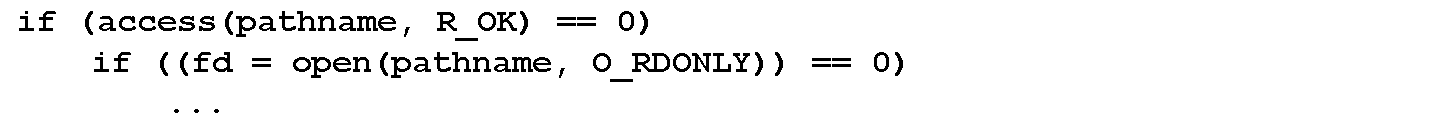
\includegraphics[width=0.47\textwidth]{figures/toctou}
%	\centering
%	\caption{The gap between access() and open() leaves the attack time window for the attacker to make changes in the file system.}
%	\label{fig:toctou}
%\end{figure}
%
%Assume this code piece belongs to a setuid program. It first validates that the ``pathname'' is readable, and if so, open the file for reading. However, the attacker can change the file system between the two system calls to trick the setuid program into opening a file that it should not.



\subsection{Kernel-level TOCTOU Vulnerability}

TOCTOU is a type of vulnerability that involves two references on the same variable or system state. The attacker usually passes the first security check with a benign value and then changes it to a malicious one before the second reference. It is a classic vulnerability, mostly amount file system APIs, which many previous research works have addressed it~\cite{dean2004fixing}~\cite{borisov2005fixing}.


TOCTOU also happens in the operating system kernel. Unlike the classic file system TOCTOU that between APIs, kernel-level TOCTOU happens within individual system calls. When a user program invokes a system call, it usually needs to provide parameters, and it is the kernel's responsibility to verify the legitimacy of the parameters and makes a kernel copy for subsequent use. However, the kernel may fail to accomplish that. Due to the developer's coding style or the unawareness of such vulnerability, the kernel routines do not use the kernel copy of user parameters and fetch the data from userspace again. Even worse, due to various reasons, a kernel module may not fully decouple with the user-mode components, and it directly uses data from userspace.


The double or multiple fetches may lead to severe issues such as local privilege escalation vulnerability. The parameter sent into the kernel is benign initially to pass the security check; then, the attacker alters it to malicious to introduce an error such as a buffer overflow to the kernel. Although the time window between two kernel fetches may be as narrow as several instructions, it is feasible to create the race condition with careful craft, especially on a multi-processor system.


Due to mistakenly repeated operations on user parameters, kernel-level TOCTOU widely exists among operating systems, even in a system such as Linux that use particular gateway functions, \texttt{copy\_to\_user()} and \texttt{copy\_from\_user()}, to get user parameters. ~\autoref{table:cves} lists a portion of recent kernel-level TOCTOU vulnerabilities.


\begin{center}
\begin{table}[ht]
%\singlespacing
%\scalebox{0.8}{
\small
\caption{Recent vulnerabilities categorized as race condition or time-of-check-to-time-of-use in the CVE database.}
\label{table:cves}
\centering
	\begin{tabular}{@{}>{\raggedright\arraybackslash}m{2.35cm}@{}|
			@{}>{\centering\arraybackslash}m{1.35cm}@{}|
			@{}>{\centering\arraybackslash}m{2.35cm}@{}|
			@{}>{\centering\arraybackslash}m{1.25cm}@{} } 
\hline
CVE-ID & Affected System & CVE-ID & Affected System \\ %[0.5ex]
\hline
CVE-2008-2252  & Windows & CVE-2016-5728 & Linux \\
CVE-2013-1280  & Windows & CVE-2016-6130 & Linux \\
CVE-2018-7249  & Windows & CVE-2020-9796 & macOS \\ 
CVE-2020-9839  & macOS   & CVE-2020-9990 & macOS \\
CVE-2016-10439 & Android & CVE-2016-7624 & macOS \\
CVE-2016-10383 & Android & CVE-2017-7115 & iOS \\

CVE-2020-5967  & Nvidia  & CVE-2020-8680 & Intel \\
\hline

\end{tabular}
\end{table}
\end{center}




\begin{figure}[th]
	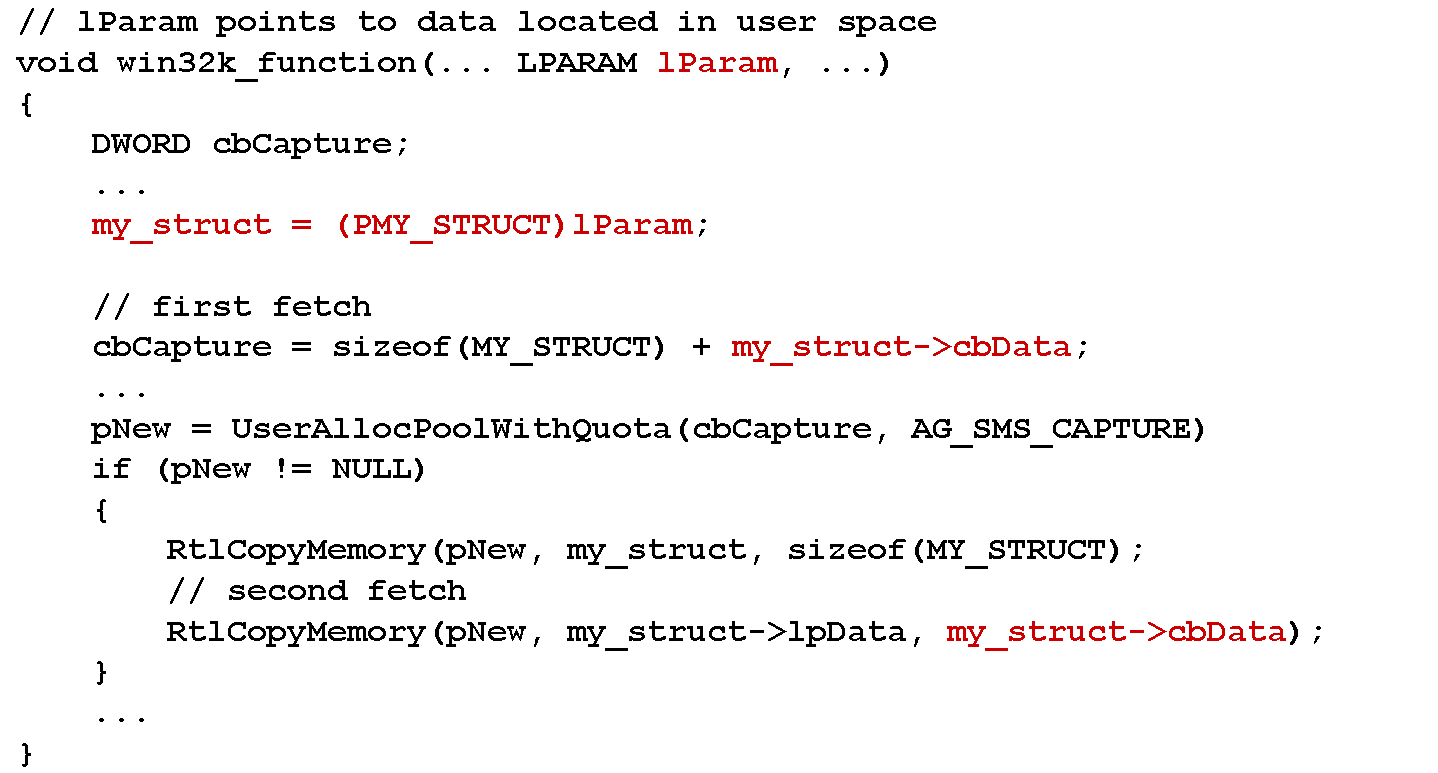
\includegraphics[width=0.47\textwidth]{figures/code08061}
	\centering
	\caption{Pseudocode of the vulnerability fixed in ms08-061. The vulnerable variable is in red. The kernel reads it twice, and it may get a different value for the buffer allocation and the subsequent buffer copying. It is common to see such a coding style. However, it is vulnerable because the two reads cross the privilege boundary.}
	\label{fig:code08061}
\end{figure}




~\autoref{fig:code08061} shows a kernel-level TOCTOU vulnerability pseudo-code from the Windows Win32k module~\cite{jurczyk2013identifying}~\cite{ms08061}. It has been identified and patched in ms08-061. The code belongs to a Win32k system call, and the red part shows the trace of the vulnerable data.  The user program passes \texttt{lParam} to \texttt{win32k\_function()} through upper layer APIs.  Adding \texttt{my\_struct->cbData} to \texttt{cbCapture} is where the kernel first gets this variable and allocates a buffer based on it. Notice, although the variable is called \textit{capture}, the developer forgot to use it subsequently.  Several instructions after, the kernel fetches this variable again when copy data into the new buffer.  An attacker can change the user variable \texttt{my\_struct->cbData} between the two fetches, especially enlarge it. Then it is a kernel buffer overflow.


~\autoref{fig:toctouasm} shows the attack.  To exploit a local privilege escalation vulnerability, the attacker can invoke the vulnerable system call as many times as needed and create another thread to race with the kernel, aiming to enlarge the data during the time window. Thread 1 keeps flipping one higher bit in the variable to make the second fetch's value larger than the first one. It succeeds by chance; otherwise, the attacker can repeat the attack.


\begin{figure}[ht]
  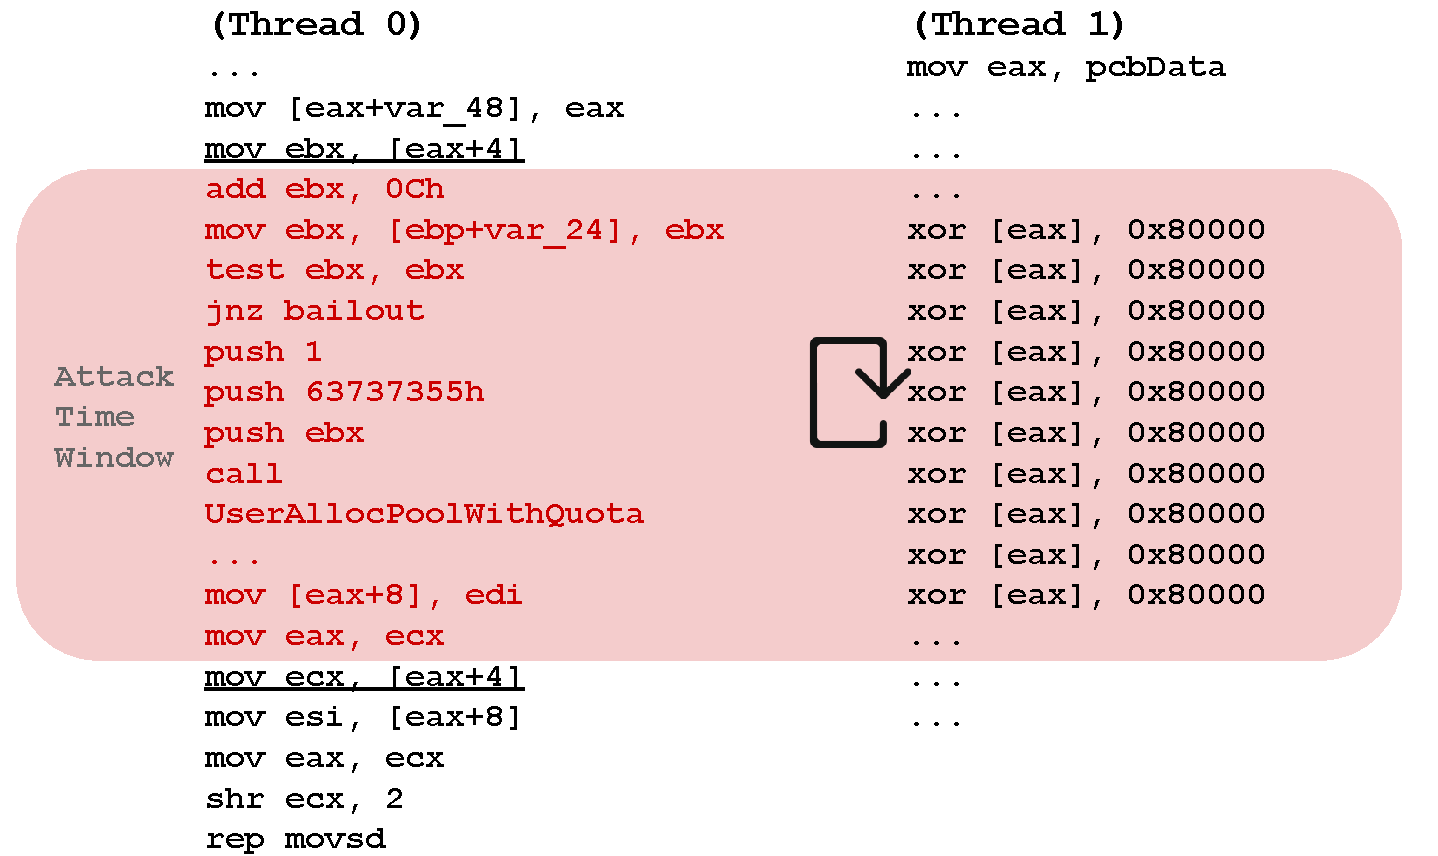
\includegraphics[width=0.47\textwidth]{figures/toctouasm3}
  \centering
  \caption{Thread 0 runs the vulnerable system call in the kernel-mode. The attacker can repeatedly call it to open the attack time window multiple times. Simultaneously, the other user-mode thread created by the attacker tries to flip the user-mode variable in-between the time window. So that the kernel code, two times, get the value differently.}
  \label{fig:toctouasm}
\end{figure}


%Once this step is accomplished, the problem becomes how to exploit it a classic heap buffer overflow. So you can see that kernel TOCTOU itself may not seems to be harmful, but it could lead to something serious. 

\subsection{Supervisor Mode Access Prevention (SMAP)}

%Kernel TOCTOU only needs accurate timing and memory writing, it's too plain to trigger any security mechanism so far. Existed monitoring methods are either too slow or too narrow, more details in~\autoref{sec:ktoctou-relatedwork}. We found a Intel CPU feature, Supervisor Mode Access Prevention (SMAP) is suitable for this task. 

%It's a security feature since Broadwell microarchitecture. It prevents operating system kernel directly accessing user-mode memory, which raises an exception. The intension is to stop transferring malicious payload from user space to kernel space.

%SMAP is enabled when the SMAP bit(21) in the CR4 is set. SMAP can be temporarily disabled for explicit memory accesses by setting the EFLAGS.AC (Alignment Check) flag. Because kennel does need to legally get data from user space, two more new instructions STAC (set AC flag) and CLAC (clear AC flag) are provided to accomplish that. The idea is that the kernel should be aware of when it's doing so. 

%For example, Linux kernel support for SMAP since version 3.7. All the accesses to user mode memory must go through two gateway functions \texttt{copy\_to\_user()} and \texttt{copy\_from\_user()}, where SMAP is temporarily disabled.

%However, Windows doesn't support SMAP yet. Different from Linux's approach, each of Windows syscalls tends to ``probe'' and ``capture'' user-mode data itself. Probing usually done by function ProbeForRead()~\cite{probeforread} and ProbeForWrite() to check the validity of the buffers, it also checks if a user mode buffer actually resides in the user space by simply compare its address to a pre-defined value. Since some modules such as win32k.sys are highly coupled with user-mode components, it will cost huge engineering effort to change the way it retrieve user-mode data.

%In Linux, even though \texttt{copy\_*\_user()} is mandated~\cite{corbet2012linuxsmap}, it still suffers from TOCTOU vulnerability such as mistake of using function \texttt{copy\_from\_user()} twice for the same variable~\cite{double-fetch-linux}. 



Monitoring the kernel's userspace behavior is essential to \name. Due to x86 protected mode characteristics, there is no mechanism available for a broad range of monitoring memory modifications. Techniques such as leveraging hardware watchpoints or transactional memory are fittable for fuzzing such vulnerabilities in a small memory range. However, none of them is realistic for run-time system protection. We discuss more details in~\autoref{sec:ktoctou-experiment} and~\autoref{sec:ktoctou-relatedwork}.

Fortunately, we notice an Intel CPU feature so-called Supervisor Mode Access Prevention (SMAP)~\cite{corbet2012supervisorsmap}~\cite{mulnix2016intel} accurately serves the purpose.
SMAP is a feature since the Intel Broadwell microarchitecture prevents the kernel from freely accessing userspace so that such access will raise an exception. It complements Supervisor Mode Execution Prevention (SMEP)~\cite{fischer2011supervisor} that introduced earlier. SMEP can be used to prevent the kernel from unintentionally executing user-mode code. SMAP extends this protection to reads and writes. It makes it harder for a malicious program to deceive the kernel into using code or data from the userspace.

SMAP is enabled when CR4.SMAP sets to 1. SMAP can be temporarily disabled for direct memory accesses by setting the EFLAGS.AC flag, and the stac and clac instructions set or clear the flag. Doing so indicates that the kernel is fully aware the userspace-access behavior. For example, Linux kernel supports SMAP since version 3.7. The kernel-to-userspace accesses must go through two gateway functions \texttt{copy\_to\_user()} and \texttt{copy\_from\_user()}, in which SMAP is temporarily disabled.

However, Windows does not support SMAP still. It takes a different approach: ``probe'' and ``capture'' user-mode data from each system call. ProbeForRead()~\cite{probeforread} and ProbeForWrite() validates user-mode buffer. It also checks whether the buffer belongs to userspace by comparing the buffer address to a pre-defined value. This mechanism is effective if done correctly and thoroughly. However, kernel components such as Win32k still failed to practice the ``probe'' and ``capture'' in a large portion of their code. Because Win32k still couples with user-mode components, it will cost huge engineering effort to change how it directly access user-mode data.

\subsection{Intel Virtualization Technology}

Intel Virtual-Machine Extensions (VMX) provides hardware-assistant virtualization, which adds 13 new instructions: VMPTRLD, VMPTRST, VMCLEAR, VMREAD, VMWRITE, VMCALL, VMLAUNCH, VMRESUME, VMXOFF, VMXON, INVEPT, INVVPID, and VMFUNC. VMX supports two modes, namely root and non-root mode, where in root mode runs the hypervisor, and virtual machines or called guest runs in non-root mode. On x86 architecture, the CPU has 4 protection rings, wherethe kernel runs at ring 0, the highest priority ring, and the user programs runs at ring 3, while the other two rings are not used. With VMX, the root model is often viewed as the ring -1. 

VMXON/VMXOFF enters/exits VMX mode. The Virtual Machine Control Structure (VMCS) is the most important data structure, which stores the data and state of one virtual CPU for one virtual machine. Each core in a physical CPU has a VMCS pointer. It points to the physical address of one VMCS. VMPTRLD loads the VMCS pointer from physical memory and makes it active and current. On contrary, VMCLEAR stores VMCS active states back to memory and makes it inactive. Although hypservisor fully aware the physical address of each VMCS but it can not modify them directly. All the operations on VMCS should go through instruction VMREAD and VMWRITE. 

The VMCS contains many data-fields that are related to aspects of a virtual machine. They are organized into six logical groups, namely, Guest-state area, Host-state area, VM-execution control fields, VM-exit control fields, VM-entry control fields, and VM-exit information fields. The last four groups compose VMX controls, which control the virtual machine's behavior such as when to exit to the hypervisor. In VMX's term, VM entry is the transition into the VMX non-root operation while VM exit is the transition from the VMX non-root virtual machine to the VMX root  hypervisor. When VM exit, the processor stores its state into the Guest-state area and loads Host-state area into hardware. In contrast, it loads Guest-state area and stores Host-state area when entering the virtual machine.

\subsection{x86 Architecture}

In this part, we briefly describe background information regarding x86 architecture. These mechanisms are more-or-less use in \name. Topics such as IPI and APIC may fall into this category loosely.

\textbf{\textit{Paging and Virtual Memory.}} On x86 architecture, with the flat or the segmented memory model, linear address space is mapped into the processors' physical memory space either directly or through paging.  Direct mapping is a one-to-one mapping between the linear address and physical address, also known as real-mode. When using the x86 paging mode, the linear address space (often referred to as virtual memory) is divided into pages. For simplicity, we only consider 4KB pages in this paper. The pages of virtual memory are then mapped as needed with physical pages.

Address translation hardware in the processor, often referred to as a Memory Management Unit (MMU), automatically translates virtual addresses to physical addresses with a data structure so-called page table. The translation creates the illusion for every process that it has a large flat virtual memory space (4GB on a 32-bit system).



\textbf{\textit{Page Table.}} The Memory Management Unit (MMU) uses page tables to map physical pages to virtual pages~\cite{intelpaging} so that each process in the system can have a flat virtual memory space. However, to store PTE, the page table's memory usage is unignorable, even on a 32-bit system with a virtual 4GB address. Therefore the page table uses a hierarchy structure to save memory. As shown in~\autoref{fig:pagetable}, the virtual address splits into three parts. The last 12-bit is the byte offset on the page, while the first two 10-bit are the index of the page table base (CR3) and Page Directory (PD). The table is composed of 4KB pages.  The system swaps out long-time unvisited page table pages to save physical memory. 

%As shown in~\autoref{fig:pte}, the least significant bit being zero indicates this page is not present in the physical memory, which brings the following issue. 

When we walk through the page table, it is inevitable to encounter an invalid page-table page, which was not a problem because the system will automatically bring it back by another page fault regarding page absence. However, this becomes a problem since we are already in the context of a SMAP page fault. The swapping process involves the system reading disk, which means more system calls. Due to the reasons mentioned above, system calls inevitably trigger more SMAP exceptions, which form a dead loop. Therefore, to solve this issue brings one of the necessities of developing a hypervisor-based solution to contain SMAP to the process level. 



\begin{figure}[th]
  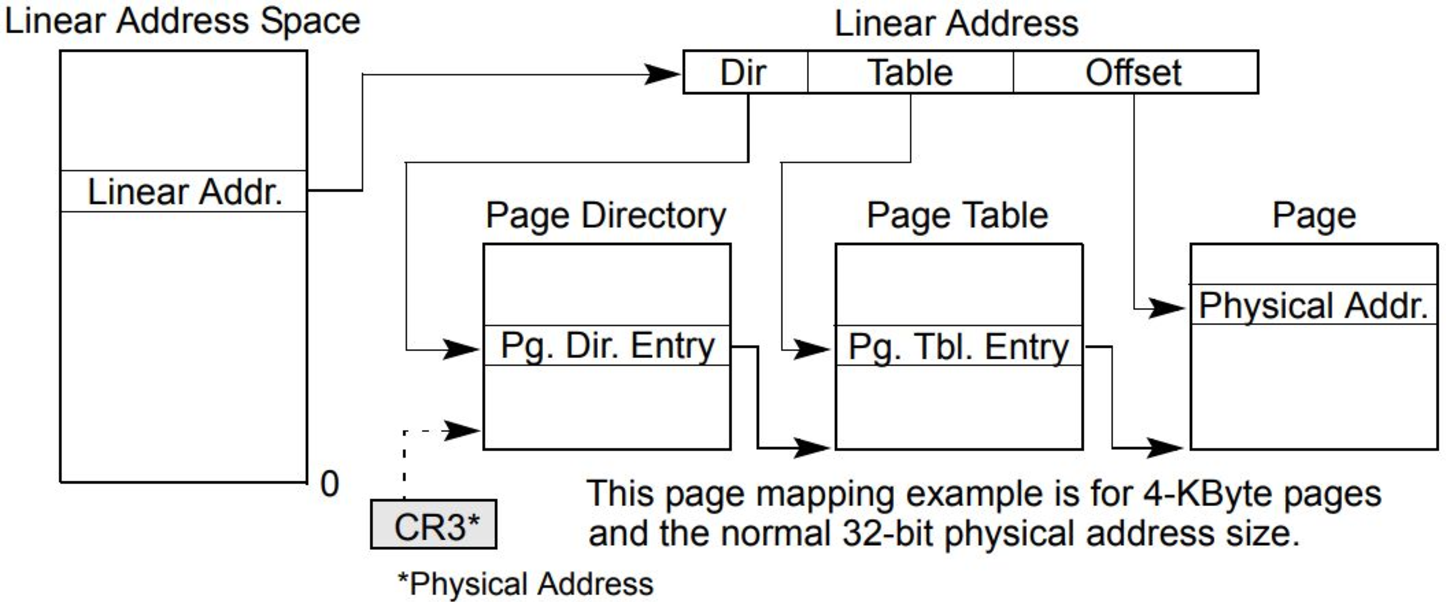
\includegraphics[width=0.47\textwidth]{figures/pagetable}
  \centering
  \caption{Linear-Address Translation to a 4-KBbyte Page using 32-Bit Paging~\cite{guide2011intel}}
  \label{fig:pagetable}
\end{figure}

\textbf{\textit{Translation Lookaside Buffer.}} As mentioned above, page table walking is a lengthy process. A full walk needs to access two pages (PD page and PTE page). If any of the two pages are not present in the memory (PDE or PTE invalid), it further triggers a page fault to bring the absent page back.

A Translation Lookaside Buffer (TLB) is a memory cache used to reduce the time for the processor to access a virtual memory address. It is part of MMU. A TLB has a fixed number of slots that stores the recent translations of virtual memory to physical memory and permission bits.  A TLB may reside between the processor and the processor cache or between the processor cache and the main memory. If valid TLB entry exists, the corresponded PTE is ignored. The system kernel is responsible for the consistency between TLB and page table.



\textbf{\textit{Interrupt Descriptor Table.}} The Interrupt Descriptor Table (IDT) is a data structure used on the x86 architecture to implement an interrupt vector table. The processor uses the IDT to determine the correct response to interrupts and exceptions. IDTR is the register on each processor to store the address of the IDT.

\textbf{\textit{Interrupts and Exceptions.}} The fundamental difference in microarchitecture between interrupt and exception is as follows.  An interrupt is an asynchronous event that is typically triggered by an I/O device. An exception is a synchronous event generated when the processor detects one or more predefined conditions while executing an instruction. However, one thing in common is that their handlers are all in the IDT, which makes them easy to confuse.

Furthermore, exceptions are classified as \textbf{faults}, \textbf{traps}, and \textbf{aborts} depending on the way they are reported and whether the instruction that caused the exception can be restarted without loss of program or task continuity. Aborts are not recoverable. They are used to report severe errors, such as hardware errors and inconsistent or illegal values in system tables. Faults and traps are recoverable, and the main difference between them is that when recovers from faults, the return address is the faulting instruction. On the other side, the trap's return address points to the instruction to be executed after the trapping instruction. In our case, the SMAP exception is a fault and handled through the page fault handler.

The IDT has 256 entries. Entry 0-31 are for exceptions except the entry 2 is for Non-Maskable external Interrupt (NMI). The rest are for external interrupt from INTR pin or INT n instruction. However, INT n also known as a software interrupt. It is essentially an exception with "interrupt" in its name, and its vector located with other external hardware interrupt vectors. Fun.



\textbf{\textit{Trap Frame.}} It is the data structure pushed to the stack by the processor. It contains registers of the current thread when an interrupt or exception occurs. Each trap frame stores only a subset of the registers depending on scenarios, namely, the SS:ESP is pushed base on if there is a change in Current Privilege Level (CPL) of the CS register.  In the context of a page fault, ErrorCode, CS:EIP, EFLAGS, and SS:ESP are pushed into the kernel stack.



\textbf{\textit{Gate.}} Code modules in lower privilege segments can only access modules operating at higher privilege segments through a tightly controlled and protected interface called a \textbf{gate}.  There are four types of gate, namely, \textbf{task gate}, \textbf{trap gate}, \textbf{interrupt gate}, and \textbf{call gate}. Fully describe and distinguish them is out of the paper's scope. The project only involves the interrupt gate.

The vectors in the IDT go through either the interrupt gate or trap gate. The difference between them is as follows. If the interrupt or exception handler is called through an interrupt gate, the processor clears the interrupt enable flag (IF) in the EFLAGS register to prevent subsequent interrupts from interfering with the execution of the handler.  When the processor invokes a handler through a trap gate, it does not change the IF flag. Having EFLAGS.IF set is a requirement to control stack depth, which also involves what type of interrupt controller installed in the system. We observed that the processor invokes the page fault handler through an interrupt gate. We think the reason for that is as follows. The processor loads the CR2 register with the 32-bit virtual address that generated the exception. Another page fault can potentially occur during the execution of the page fault handler. Hence the page fault handler should save the contents of the CR2 before a second page fault can occur because the processor update CR2 whenever a page fault is detected.

\textbf{\textit{CS Segment and Current Privilege Level}} CS segment register cannot be set directly through instruction mov, unlike other segment registers,  but only through a trap or interrupt gate. The system's current privilege level depends on the Current Privilege Level (CPL) field in the CS segment, which is maintained by the processor. This 2-bit CPL field in the code segment register is always equal to the processor's current privilege level. When getting the CS image from the trap frame of a page fault context, it provides us the ground truth of what privilege of the code when the SMAP exception happens, so that we do not make the decision based on the apparent value of EIP. To fully explain the privilege transition mechanism is out of the paper's scope.

\textbf{\textit{Inter-processor Interrupt.}}  It is an interrupt controller mechanism to interrupt another processor or group of processors on the system bus. They are used for software self-interrupts, interrupt forwarding, or preemptive scheduling. In \name, we use IPI to flush TLB cache on all the processors.

\textbf{\textit{Local APIC.}} Intel's Advanced Programmable Interrupt Controller (APIC) is a family of interrupt controllers. It is more advanced than Intel's 8259 Programmable Interrupt Controller (PIC). Nowadays, SMP systems with multiple processors utilize APIC. The APIC is a split architecture design, with a local APIC usually integrated into the processor and an optional I/O APIC on a system bus. The local APIC performs two primary functions for the processor:
It receives interrupts from the processor's interrupt pins, internal sources, and an external I/O APIC. It sends these to the processor core for handling.
It sends and receives IPI messages to and from other logical processors on the system bus in multiple-processor systems.
The external I/O APIC is part of Intel's system chipset. It is responsible for receiving interrupts generated by system hardware and I/O devices and forwarding them to the local APIC as interrupt messages. A processor can generate IPIs by programming the interrupt command register (ICR) in its local APIC. Writing to the ICR generates an IPI message on the system bus or the APIC bus. When the target processor receives an IPI message, its local APIC handles the message automatically using information included in the message such as vector number and trigger mode. The IPI mechanism sends interrupts for a specific vector number, and special-purpose interrupts to processors on the system bus. Local APIC registers are memory-mapped to a 4-KByte region of the processor's physical address space with an initial starting address of EFF00000H. The software interacts with the local APIC by reading and writing its registers. It also can change the initial mapping to a different 4-KByte region for all the local APICs. The presence of a local APIC can be detected using the CPUID instruction. Execute CPUID with source operand of 1 in the EAX register, then bit 9 of returned feature flags in EDX register indicate a local APIC.


\begin{figure}[th]
  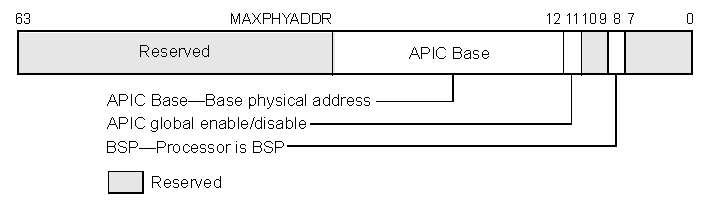
\includegraphics[width=0.47\textwidth]{figures/ia32apicbase}
  \centering
  \caption{\texttt{IA32\_APIC\_BASE MSR}}
  \label{fig:ia32apicbase}
\end{figure}

There is only one MSR associated with local APIC, \texttt{IA32\_APIC\_BASE}. As shown in~\autoref{fig:ia32apicbase}, the BSP flag indicates if the processor is the bootstrap processor (BSP); ``APIC global enable/disable'' enables/disables the APIC; APIC base specifies the base address of the APIC registers. This 24-bit value needs to be extended by 12 bits at the low end to form the base address. As formerly mentioned, this value by default is 0xFEE00000.

The primary local APIC facility for issuing IPIs is the interrupt command register (ICR), as shown in~\autoref{fig:icr}. It is a 64-bit local APIC register that allows the operating system to specify and send IPIs to processors in the system.


\begin{figure}[th]
  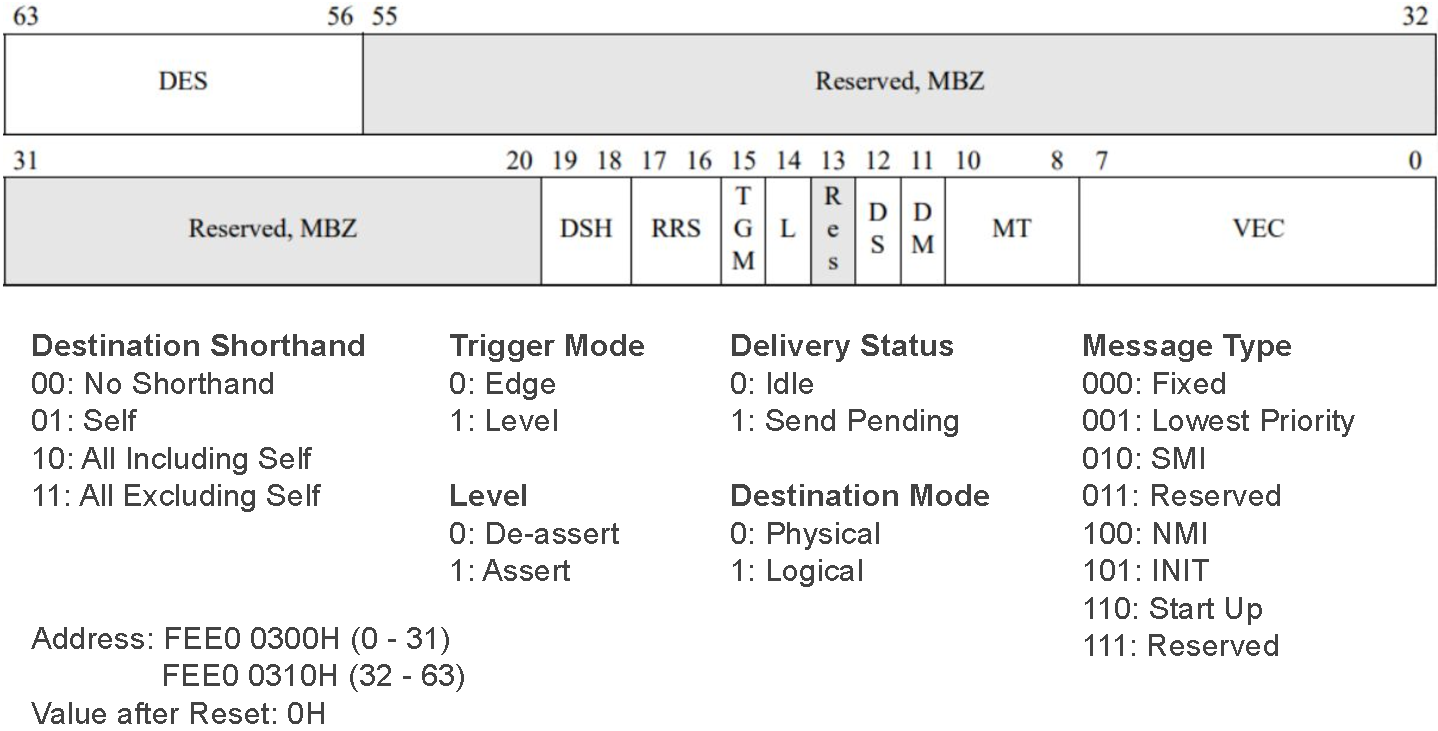
\includegraphics[width=0.47\textwidth]{figures/icr2}
  \centering
  \caption{Interrupt Command Register (ICR). Notice, Intel and AMD has slightly different definitions.~\cite{intelapic}~\cite{amdapic}}
  \label{fig:icr}
\end{figure}


\section{Overview}
\label{sec:ktoctou-overview}




\subsection{Threat Model}
\label{sec:ktoctou-threatmodel}

Kernel TOCTOU is a local privilege escalation vulnerability. The vulnerability could allow local users or malicious software to gain full root privileges. We assume an attacker has a user account that can upload and run arbitrary programs with user privilege, or he can access such a program. The attacker has arbitrary memory read and writes primitives. He is also able to call any system services or load any library. The DEP policy (\textbf{W}rite $\oplus$ e\textbf{X}ecute) and ASLR is not necessary. We assume the attacker has full knowledge about the system kernel, including the memory layout. However, he can not read or write any kernel memory as a classical operating system would not allow. The attacker aims at running arbitrary code in the kernel, hence obtain the highest privilege. 

We aim at the Windows OS, a complicated operating system. \name will not work on the Linux kernel because it already utilizes the Intel CPU feature SMAP in a conventional way. We will elaborate on this in~\autoref{sec:ktoctou-background}.

%Without investigation,  we can not be sure that the mitigation will work on other OS, even the underlying mechanism should work.\hb{you dont need to write this in the threat model} 

Considering we leverage a hardware feature from Intel CPU, The host system should use Intel CPU with SMAP capability.


\subsection{High-Level Design and Challenges}

The kernel double fetching a user address may cause a TOCTOU vulnerability. From a practical point of view, we can not make the kernel change its double-fetch behavior. Instead, we want to make the two fetches always get the same value, thus no vulnerability. The high-level idea is as follows.  When the kernel accesses a user address, we froze the containing page so that no other user thread can overwrite it.


The main challenges are:

\begin{itemize}
	\item How can we know when the kernel accesses a user address?
	\item It is overkill to froze an entire page just for one variable, and reads should allow.
	\item The two fetches should happen within a short time, more specifically, within the same system call. 
	\item Windows is a complex operating system, if not the most complex system. How is it practical to enable a system-wide hardware feature such as SMAP without crash the system?
\end{itemize}


\subsection{Approach Overview}


When the kernel accesses a user address, how to get notified is the most challenging issue. Because the processor reading memory is such an ordinary operation, no official hardware feature is available for monitoring that in a broad range of memory. We abuse a hardware feature SMAP. It was initially designed to prevent the attacker from tricking the kernel into getting shellcode or malicious data from userspace. However, one main character of this feature is that when the kernel accesses a user address, the processor raises a page fault exception. This part accurately serves our purpose, so we want to leverage it in a novel way.

Subject to the x86 architecture, the protection has to base on a page granularity. To protect even one byte, we have to deal with an entire page.
First, we separate the subsequent user reads from writes. The reads are harmless.  When we temporarily release a page, we also set this page as read-only to ensure no writing. When a user writes on the protected page, we make the thread suspend on the writing instruction and wait until the current system call ends.

As previously mentioned in ~\autoref{sec:ktoctou-background}, the kernel-level TOCTOU problems happen inside individual system calls. We hook Windows internal functions to known when a system call ends and release the pages the system call accessed. Also, we monitor the creation and termination for both processes and threads and use Windows internal data structures to distinguish each thread, namely, TEB.

We develop a light-weight hypervisor to confine the SMAP feature into specific processes. It makes debugging less painful to us, and it is also necessary to prevent nested SMAP exceptions that cause a dead loop.

~\autoref{fig:ktoctou-overview} shows the high-level overview. The hypervisor enables SMAP in one process, that is, the current one in the figure. The kernel accessed three user pages, as marked in the user process memory space. One user thread in the same process tries to access those pages. The read is allowed, where the page is released and set read-only. However, the write is not allowed for the moment; the page fault handler suspends the write to avoid any data inconsistency in the kernel.


\begin{figure}[th]
  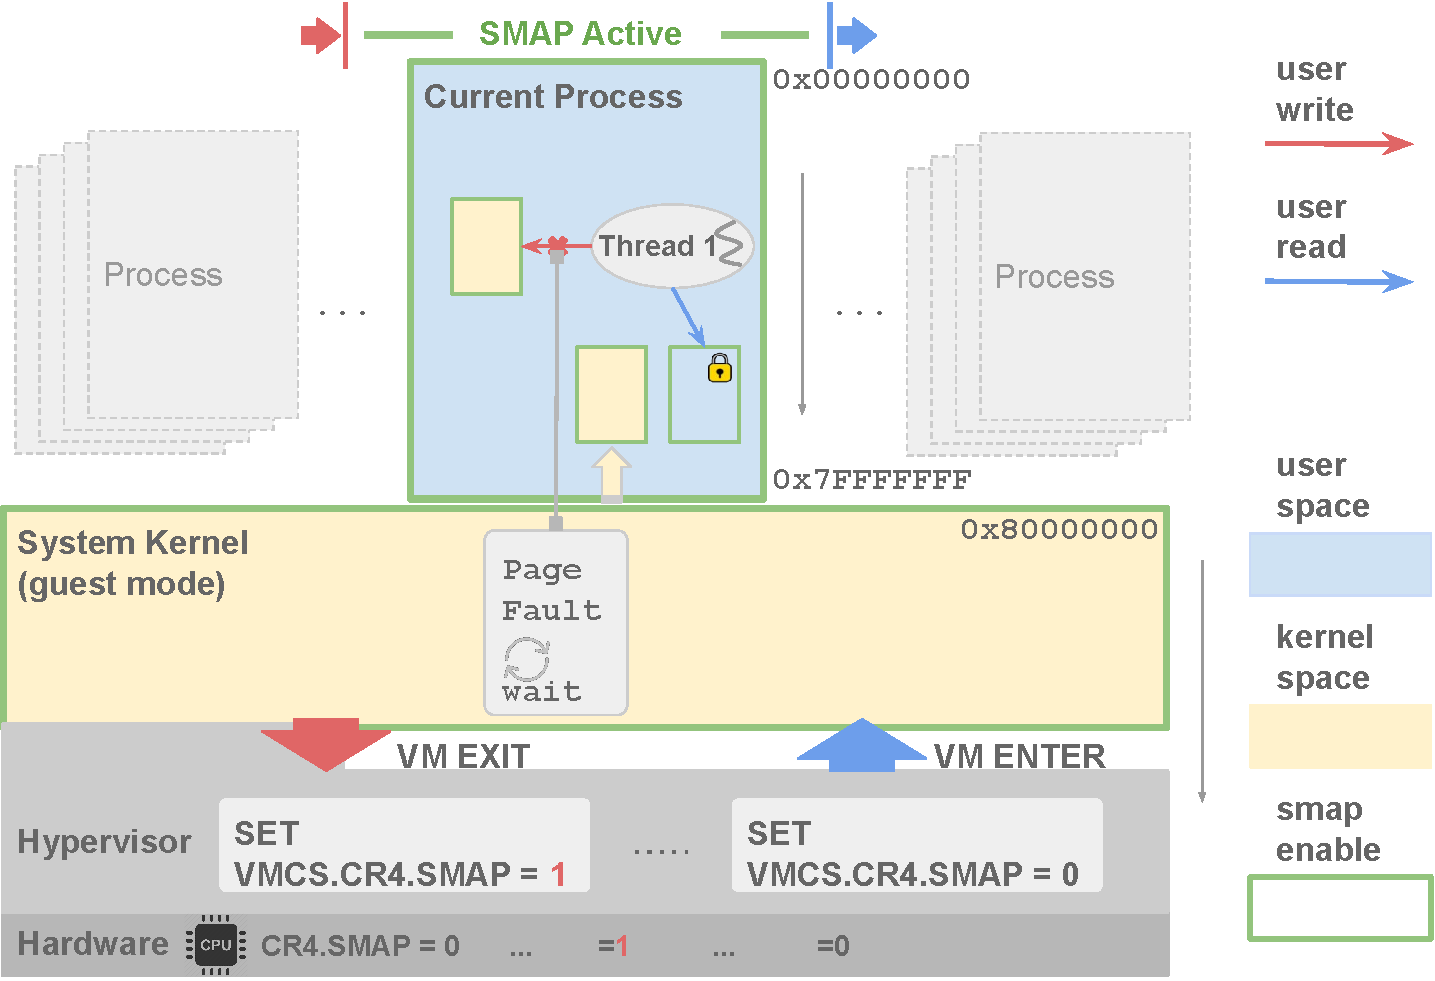
\includegraphics[width=0.47\textwidth]{figures/ktoctou-overview2}
  \centering
  \caption{The hypervisor is capable of confining the system-wide feature SMAP into one process. When the hypervisor catches the process context switch events, it changes the SMAP enable bit in the CR4 register to only set during the target process. The processor raises page fault exception when the kernel accesses userspace so that we can protect those pages. Thread 1 can read a protected page but can not write. The read is allowed by automatically setting the protected page back to userspace with a read-only permit. However, when the write instruction raises an exception, the page fault handler suspends the thread until the system call ends.}
  \label{fig:ktoctou-overview}
\end{figure}

%! TEX root = 'main.tex'
\section{Finding Kernel TOCTOU Bugs}
\label{sec:experiment}
\hb{you need to rewrite this part, I did not get what you want to tell reader. You have to summarize what you will talk in this paragraph first, then goes with the logic, what did you find, how, what are the challenges and how do you solve it smartly }One side-project is to find TOCTOU bugs, which is also essential to expose this type of vulnerability.  Previous work such as~\cite{jurczyk2013identifying}~\cite{bochspwnreloaded} utilize a full software emulated virtual machine Bochs~\cite{lawton2003bochs}. It parses and executes each instruction without hardware virtualization assistant or dynamic binary translation.  It is straight forward to instrument the operating system kernel, and it discovers many vulnerabilities of this type~\cite{jurczyk2013identifying}~\cite{bochspwnreloaded}. However, due to the nature of full software emulation, the virtual machine runs extremely slow. Therefore it is not easy to make a comprehensive test, especially with GUI programs, because it needs a prompt response.

As previously discussed, the SMAP feather is an ideal way of monitoring kernel-to-user-memory behavior. The goal is to check if the same address is being read twice by one system call. However, with the mechanism previously described, once the system protects a user-mode page by setting it to the kernel-mode, the system will not raise the SMAP exception again, which will miss the subsequent kernel accesses. Therefore, instead of protecting a page, we only want to record the information and let the system continue. Unfortunately, we tried different methods to cancel a SMAP exception, and setting the faulting page to kernel-mode is the only way that satisfies the CPU so far. Hence we want to set the protected page back to the user-mode as soon as possible not to lose track of the kernel. 

\textbf{\textit{Single Step Trap.}} It is the soonest way to get back the control. Through setting the trap flag (TF) in the EFLAGS register, the processor will stop at every instruction. We want to stop at the next instruction that follows the one that triggers the SMAP exception, set back the protected page to user-mode, and continue the kernel. The processor automatically sets the resume flag (RF) in the EFLAGS image on the stack before entry into any fault handler so that the handler will not be interrupted on every instruction. Also, the IRET instruction at the end of the handler should set the RF in the EFLAGS register, so the processor will not generate another trap at the same address. Since we have a hypervisor, the single-step trap triggers a VM exit as a non-maskable interrupt. In the event handler, we clear the TF and set the RF in the guest EFLAGS. Then the hypervisor resumes the guest virtual machine.

\textbf{\textit{Breakpoint}} Nevertheless, the single-step trap still comes in. We decide to write a software breakpoint directly on the first byte of the next instruction. After handling the user-mode page in the SMAP exception handler, we parse the current instruction to get its length. Then we temporarily disable the write protection of the kernel through set CR4.WP and we next write a byte 0xcc to the beginning of the next byte. After that, we record the information of this access and let the kernel continue. When the hypervisor gets the debug trap, we replace the missing byte, release the protected page, and then resume the virtual machine to re-run the faulting instruction. We observe that when the trap happens, in the hypervisor event handler's context, the CR3 register always has the page table base of the SYSTEM process. We need to change it to the target process and then write the missing byte to the right memory space.

\textbf{\textit{Results.}} 
We found a few double fetch bug candidates, and~\autoref{table:doubleread} in~\autoref{sec:evaluation} gives a glimpse of the problem. This method has an advantage over the binary static analysis. Different code segments may use different addressing modes with different bases to access a user-mode address.  It is not obvious to spot if the code segments are slightly apart. For example, in~\autoref{fig:doublefetch}, it needs to trace both ECX and EDX registers and, in some cases, need to get user input to calculate the address. With our solution, it is easy to spot the address after computation at run time.

\begin{figure}[th]
  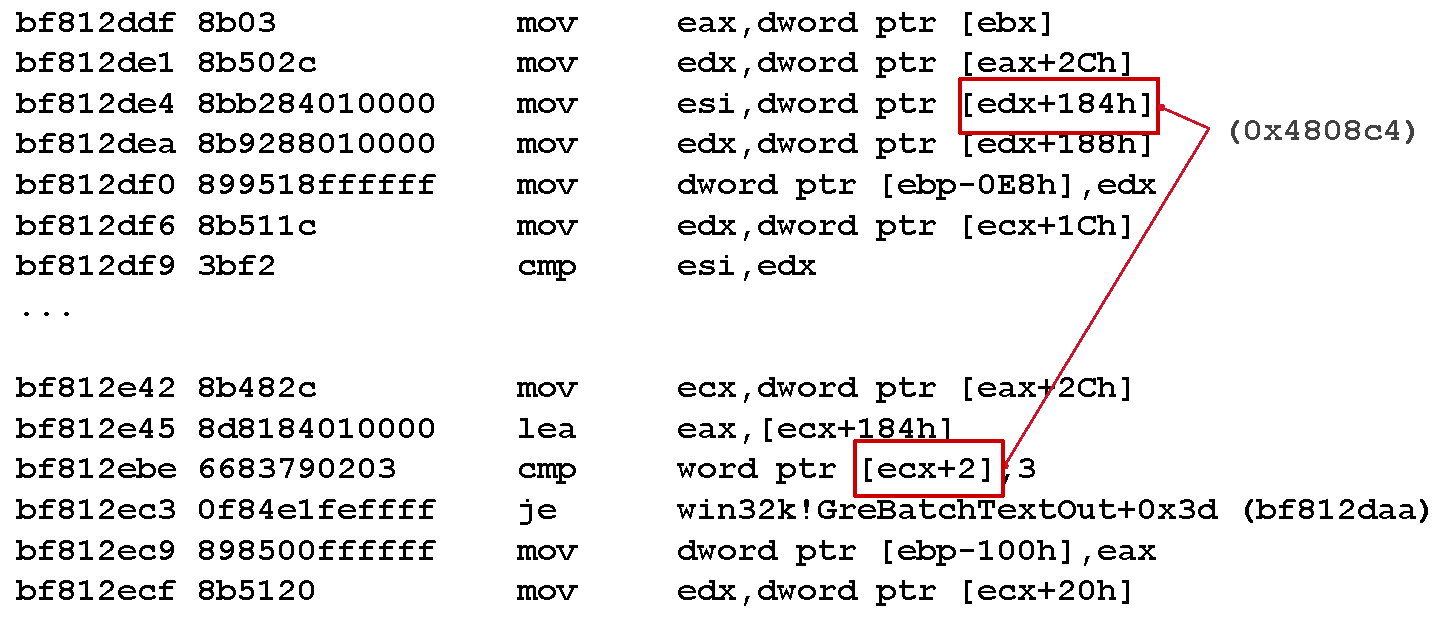
\includegraphics[width=0.47\textwidth]{figures/doublefetch}
  \centering
  \caption{CR3 0x6d40320; TEB 0x7ffdd000; EIP 0xbf812de4 and 0xbf812e4b read the same user-mode address 0x4808c4 within one system call.}
  \label{fig:doublefetch}
\end{figure}


Whether or not those bugs can further turn into vulnerabilities are case by case. However, a significant potential of those accesses is direct without a try-catch block. It may lead to a local denial-of-service (DOS) attack if the attacker can free the user-mode page right in front of the access. 

%! TEX root = 'main.tex'

\section{\name Design}
\label{sec:ktoctou-design}

This section presents the design of \name.  The core of \name includes two key components, the system module, and the hypervisor. The system module intercepts the system's page fault handler to process SMAP and relevant exceptions, which is the protection's main logic. The lightweight hypervisor puts the system into the virtual machine. Its primary use is to confine the system-wide feature SMAP into specific processes.

\subsection{System Module}

The system module's core functions include enabling SMAP, recovering from SMAP exceptions, protecting pages, and solving read/writes conflicts. We describe each technique as follows.


\textbf{\textit{Monitoring Kernel to Userspace Access. }} The biggest challenge we confront is how to monitor the kernel-to-userspace behavior efficiently. Accessing memory is such an ordinary operation so that no purposeful hardware feature is available for monitoring that.  We notice a rarely mentioned hardware feature SMAP. Its initial design prevents the attacker from tricking the kernel into getting shellcode or malicious data from userspace. When the kernel accesses a user address, the processor raises a page fault exception. This part accurately serves our purpose, so we want to leverage it in a novel way.

However, not every aspect of this feature perfectly fits our exceptions. If in an ideal situation, the hardware should report on each kernel-to-userspace access and freeze the user memory at machine word granularity. In reality, SMAP only works on the page level, and the exception that it raised is fatal to the system, meaning the operating system should crash when it receives such exceptions.  We eventually find a way to recover it. We intercept the system's page fault handler to handle such exceptions. Since Windows does not support SMAP, we do not pass those exceptions to the kernel. Considering the violation of raising a SMAP exception is that the kernel accesses userspace, so puts the corresponding page into kernel space does the opposite, thus solve the violation. Otherwise, it is then too late to disable SMAP through CR4 or EFLAGS.AC.


Putting a page into the kernel not only solves the exception but also protects the page. The user threads no longer can access it, which prevents the race condition between the kernel and user threads. However, it is overkill to protect the entire page and block benign reads and writes on the rest of the data. We will elaborate on the read/writes conflicts in the following sections.



\textbf{\textit{Solving Read Conflicts}}. For practical purposes, solving
read conflicts is essential. It is common to have multiple global
variables or multiple heap buffers share the same page. Therefore, when we protect an entire page, we block benign access to the rest of the data. It is especially unnecessary because reads do not harm security.

We solve the read conflicts by setting the protected page
back to userspace, allowing user threads to read. When user threads read a kernel-mode protected page, the processor raises an exception due to the privilege violation. Therefore our page fault handler gets the notification and sets the page back to userspace. Additionally, the page is also set with a read-only permit to ensure no write. ~\autoref{fig:pagestate} shows the transitions between kernel-mode and user-mode.  We record the original page information to handle various situations and correctly restore it at the end of the system call.


\begin{figure}[th]
  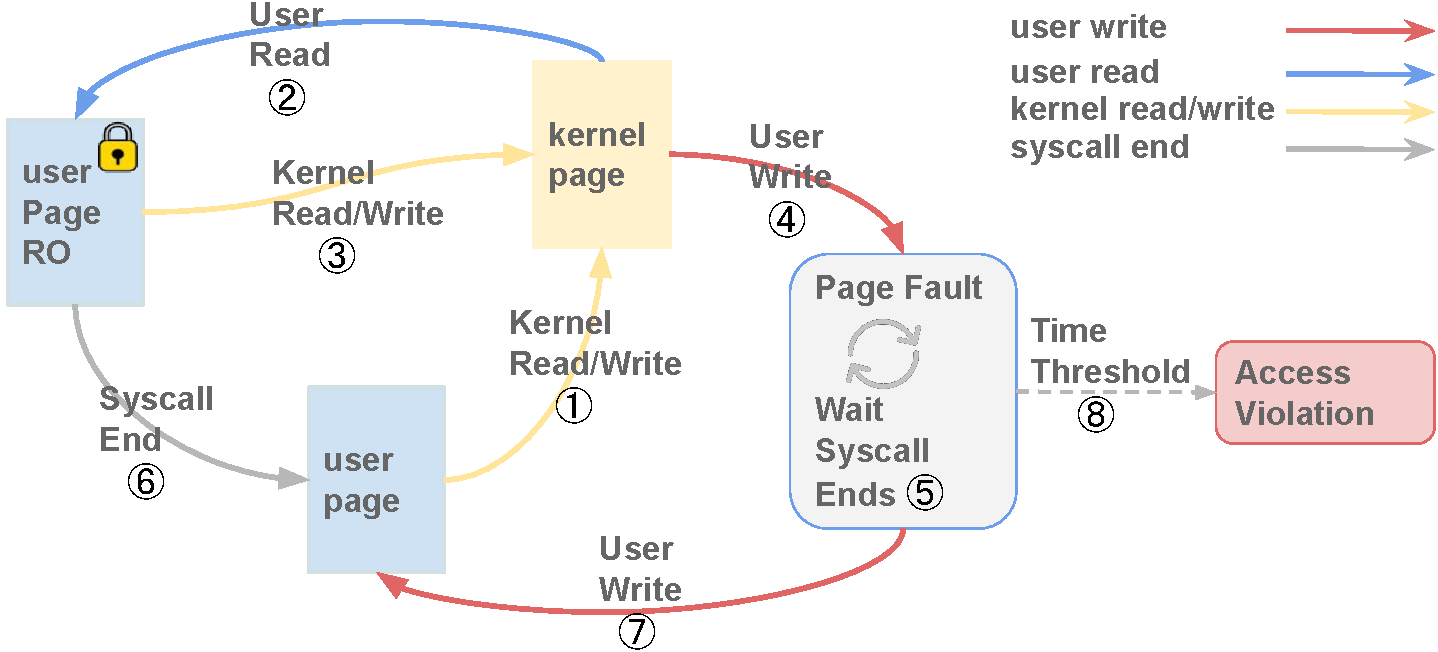
\includegraphics[width=0.47\textwidth]{figures/pagestate6}
  \centering
  \caption{Page attributes transits in different states. A user page becomes a kernel page when the kernel read/write it~\texttt{\textcircled{1}}. Afterward, if user threads read this page, our page fault handler changes it back to user-mode with a read-only permit~\texttt{\textcircled{2}}. This page is again capable of triggering a SMAP exception if the kernel reaccesses it~\texttt{\textcircled{3}}. Our page handler suspends any user thread that tries to write a protected page~\texttt{\textcircled{4}}. It then calls a sleep function, letting the operating system, and wakes up periodically to check the page's status~\texttt{\textcircled{5}}. When the current system call ends, this page is restored to user-mode with its original permits~\texttt{\textcircled{6}}. The write thread is also released and re-execute the faulting instruction to write the page~\texttt{\textcircled{7}}. However, if the thread waits too long, it will be terminated to avoid a deadlock~\texttt{\textcircled{8}}.}
  \label{fig:pagestate}
\end{figure}




\textbf{\textit{Page Attribute Transition.}}  The modifications on the page attributes are essential to this mitigation. Because changing a user page to kernel-mode is the primary method of protection.  Moreover, to solve reads conflicts, we need to change the page back and forth between kernel-mode and user-mode.

First, we need to locate the page's Page Table Entry (PTE). As mentioned in~\autoref{sec:ktoctou-background}, with paging, every page in the virtual memory has an entry in the page table.  As shown in~\autoref{fig:pte}, the User/Supervisor decides whether this is a kernel page or a user page where set if a user page, otherwise a kernel page.

\begin{figure}[th]
  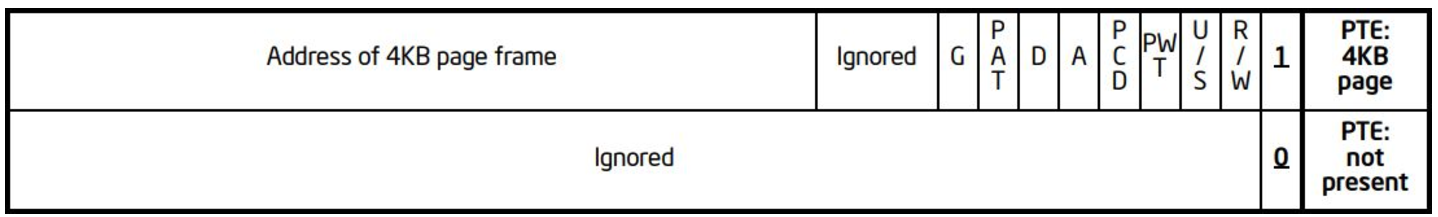
\includegraphics[width=0.47\textwidth]{figures/pte2}
  \centering
  \caption{\textbf{Bit 0} (Present): \textbf{0} indicates an invalid page. \textbf{U/S} (User/Supervisor): \textbf{0} user-mode accesses are not allowed to the page referenced by this entry. \textbf{R/W}: \textbf{0} writes are not allowed to the page.}
  \label{fig:pte}
\end{figure}



We obtain various information in the context of the page fault handler to find the corresponding PTE. The CR2 register stores the faulting virtual address. Regarding SMAP, it is the user address that the kernel accessed. The CR3 register stores the physical address of the current page table base. The trap frame in the kernel stack contains the error code, CS: EIP, SS: ESP, and EFLAGS, which describes the processor context when the exception happens.

Changing the U/S bit in the PTE makes the user page becomes a kernel page. It is counterintuitive because we usually have the impression that the virtual address between 0x80000000 to 0xFFFFFFFF is the kernel space on Windows 32-bit system. However, the processor mechanism defines the kernel space as follows. There is the Current Privilege Level (CPL) field in the CS segment. The processor maintains this 2-bit field to equal the processor's current privilege level. Meantime, the U/S bit in the PTE decides whether the unprivileged code can access it. Traditionally, we consider the memory space that only the most privileged code (CPL:00) can run as the kernel space. Indeed, it is a considerably complicated mechanism involving more data structure in the processor's microarchitecture, out of this paper's scope. In essence, the U/S bit decides whether the page is a kernel page or a user page, even the virtual address is below 0x80000000.


\begin{figure}[th]
  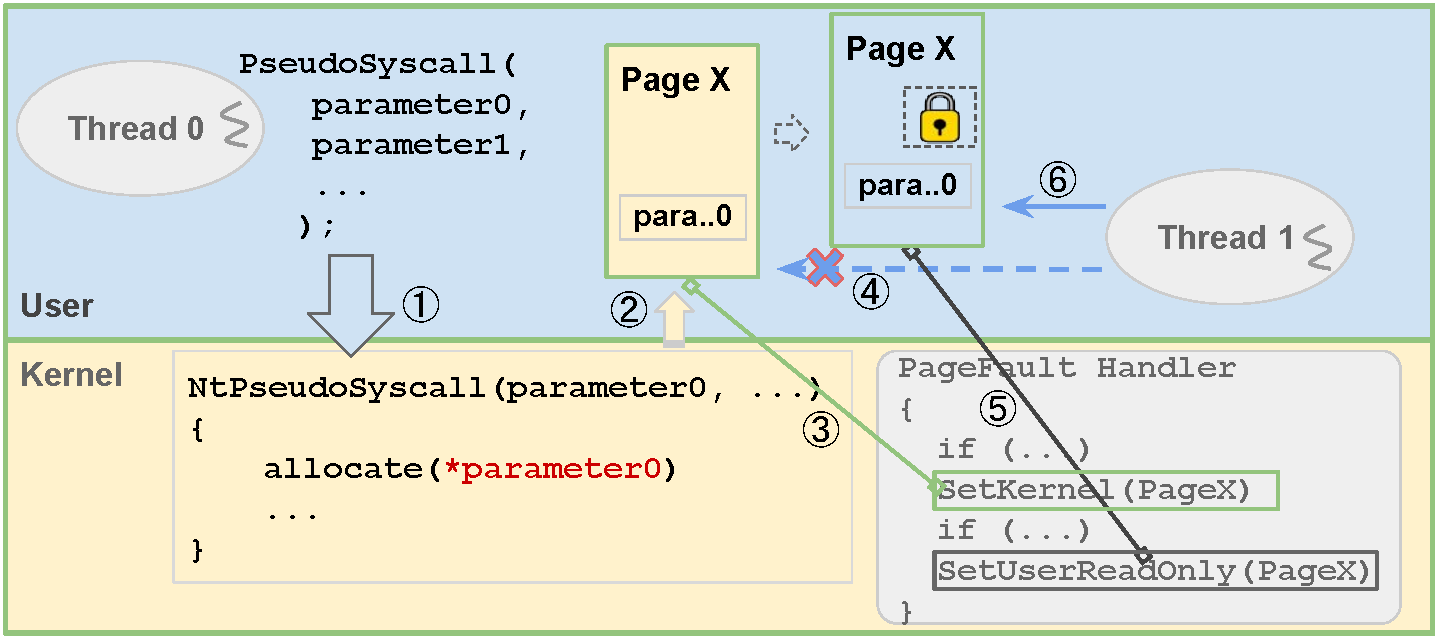
\includegraphics[width=0.47\textwidth]{figures/denyuserwrite3}
  \centering
  \caption{\texttt{\textcircled{1}} User thread 0 invokes a system call with parameters. \texttt{\textcircled{2}} The kernel fetches one of the parameters from userspace hence triggers a SMAP exception. \texttt{\textcircled{3}} Our page fault handler converts the page into kernel-mode to protect it. \texttt{\textcircled{4}} User thread 1 tries to read the protected page and triggers an exception due to privilege violation.  \texttt{\textcircled{5}} Again, our page fault handler processes the exception and converts the protected page back to user-mode with a read-only permit. \texttt{\textcircled{6}} The faulting instruction re-execute, and the user thread successfully read the data without knowing the previous exception.}
  \label{fig:denyuserwrite}
\end{figure}



~\autoref{fig:denyuserwrite} shows the mitigation convert a low address user page into a kernel page. It is a common situation where user programs invoke a system call and provide parameters. After that, if a user thread accesses a protected page, the processor raises an exception due to the privilege violation. The page fault handler converts this page to user-mode and read-only.



\textbf{\textit{Solving Write Conflicts.}} We can not allow any user code to write a protected page during its protection,  because unlike reads, the write operation is a security threat. Subject to the x86 architecture, the protection has to base on the page granularity, so not all the writes on this page will cause a TOCTOU problem. Therefore, we can not directly terminate every user thread that accesses a protected page from a compatibility perspective. To solve this, we choose to delay the write operation. After the writing instruction caused an exception, our page fault handler suspends the user thread until the end of the system call. Therefore, the protected page remains the same for the kernel, and user threads can also write it after the system call.  We explain the practicality of suspending a thread in the context of page fault in the following section.


\begin{figure}[th]
  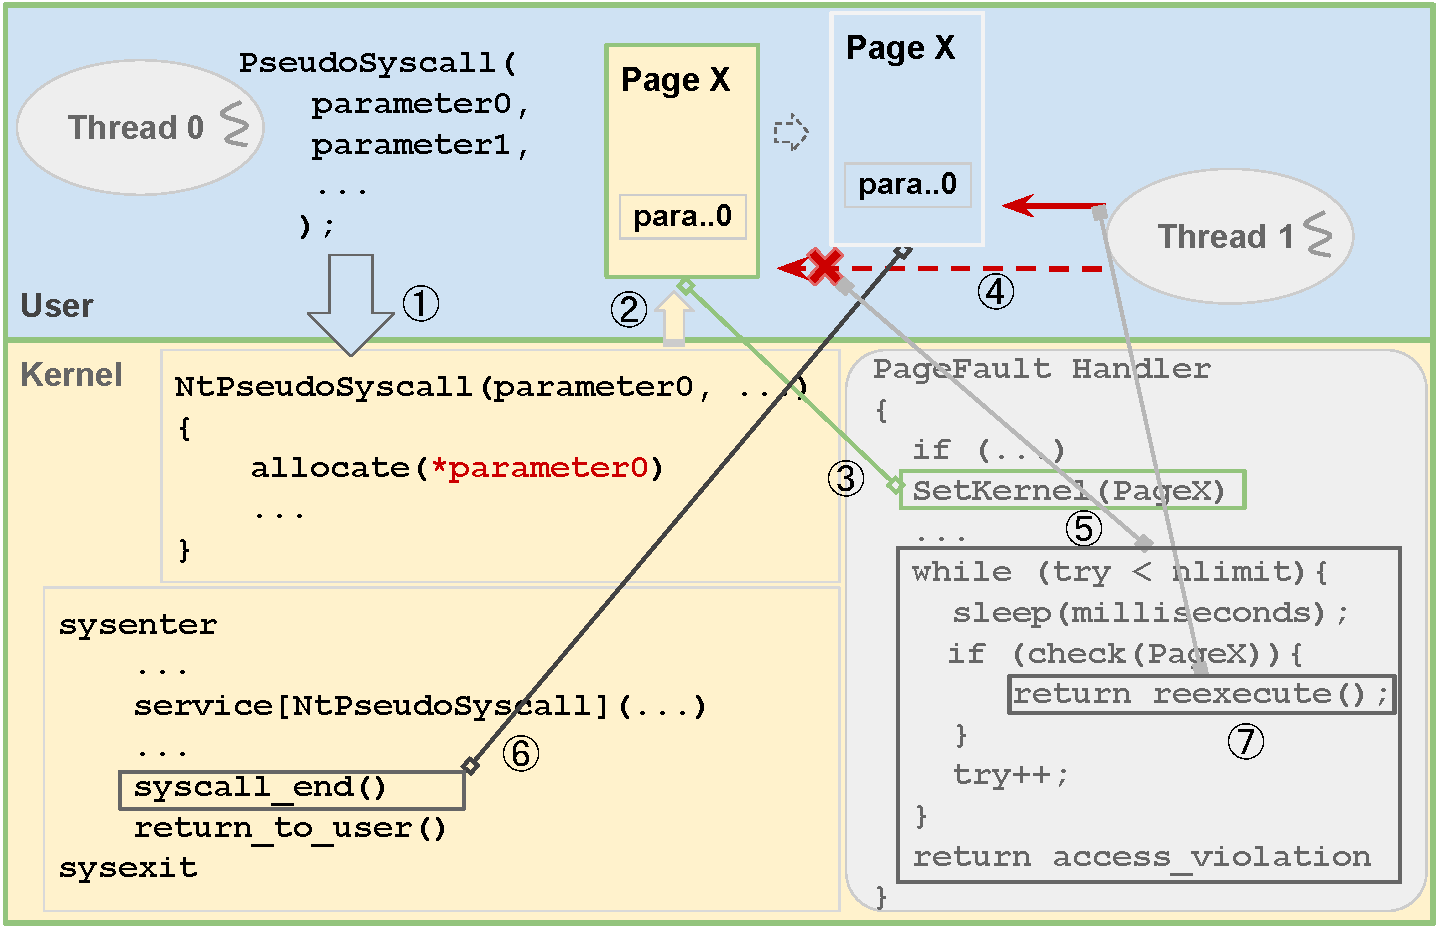
\includegraphics[width=0.47\textwidth]{figures/reexecute2}
  \centering
  \caption{To solve this, we choose to delay the write operation. \texttt{\textcircled{1}}  User thread 0 invokes a system call with parameters. \texttt{\textcircled{2}} The kernel fetches one of the parameters from userspace hence triggers a SMAP exception. \texttt{\textcircled{3}} Our page fault handler converts the page into kernel-mode to protect it.  \texttt{\textcircled{4}} User thread 1 tries to \textbf{write} the protected page and triggers an exception due to privilege violation. \texttt{\textcircled{5}} This time, our page fault handler suspends the thread by calling a sleep function, letting the operating system schedule.  It rechecks the page's status periodically when it wakes up. \texttt{\textcircled{6}} When the current system call ends, the mitigation releases all the protected pages related to this thread. \texttt{\textcircled{7}} Meantime, the page fault handler wakes up and realize that the page is released. Therefore it finishes the exception by executing the faulting instruction again.}
  \label{fig:reexecute}
\end{figure}



~\autoref{fig:reexecute} shows that thread zero invokes a system call with parameters. The kernel gets the user parameter so that the corresponded page is protected. Afterward, user thread one tries to write the page, which raises a page fault exception due to privilege violation. The page fault handler suspends the current thread by calling a sleep function, namely, \texttt{KeDelayExecutionThread()}. The thread wakes up periodically to check whether the page is released. If so, the exception is finished and re-executes the faulting instruction. Otherwise, the page fault handler may terminate the thread to prevent a deadlock if it takes too long.



\textbf{\textit{Interrupt and Exception.}} Suspending a thread inside the page fault handler seems unusual because the page fault exception resides in the Interrupt Descriptor Table (IDT) with interrupts, and they seems to be time-critical routines. However, there is an essential difference between an exception and an interrupt. An interrupt is an asynchronous event that is typically triggered by an I/O device. An exception is a synchronous event generated when the processor detects one or more predefined conditions while executing an instruction. Interrupts have a higher priority than the operating system's scheduler and most of the kernel components. Any job that takes too much time should not be processed in an interrupt handler~\cite{msdnwatchdog}.  On the contrary, exceptions have the lowest priority in the kernel. In Windows' term, the Interrupt Request Level (IRQL) that the exception handler executes at is \texttt{PASSIVE\_LEVEL}, meaning call for thread scheduling is plausible.



\textbf{\textit{Releasing Protected Pages.}} To be aware of when a system call ends, we choose to intercept Windows internal functions. We keep tracking the page table base and Thread Environment Block (TEB) to distinguish each thread, thus release the protected pages on a thread basis.


\textbf{\textit{Flushing TLB.}} We need to flush Translation Lookaside Buffer (TLB) to ensure that the page attributes modification is effective on all processors of the system. TLB is a memory cache that stores the recent translation of virtual memory to physical memory. It accelerates the process of accessing virtual memory. Different than data cache, TLB is not entirely transparent to the operating system. When the operating system updates a page table, the corresponding TLB entries need to be invalidated to get new ones. As mentioned above, we leverage the page attribute transition as the main page protection. It is critical to ensure the PTE modification takes effect instantly, especially on a multi-processor system. We examine the method to flush the TLB through local APIC as described in~\autoref{sec:ktoctou-background}. Eventually, we find Windows internal functions that flush TLB entries on all the processors. Therefore we use them and do not have to consider the underlying hardware differences.


\subsection{Hypervisor}


The hypervisor plays an essential role in developing and debugging for \name. When we first enabled SMAP in Windows, instantly, an enormous amount of exceptions flooded the system. The debugger was frozen.  It is not surprising because we know that SMP is a system-wide feature, and Windows does not support it. A significant portion of the system calls fetches user-provided parameters and system data such as Process Environment Block (PEB), \texttt{USER\_SHARED\_DATA} mapped in userspace, which all trigger SMAP exceptions.

Due to Intel VT virtualization technology's design~\cite{neiger2006intel}, it is possible to load a light-weight hypervisor as a kernel module during run time. Unlike other commercial hypervisors such as Xen, Hyper-V, and VMWare, it does not emulate hardware devices. It merely put the operating system into VM guest mode, and itself becomes the hypervisor, thus monitors system events~\cite{howtohide}.

\begin{figure}[th]
  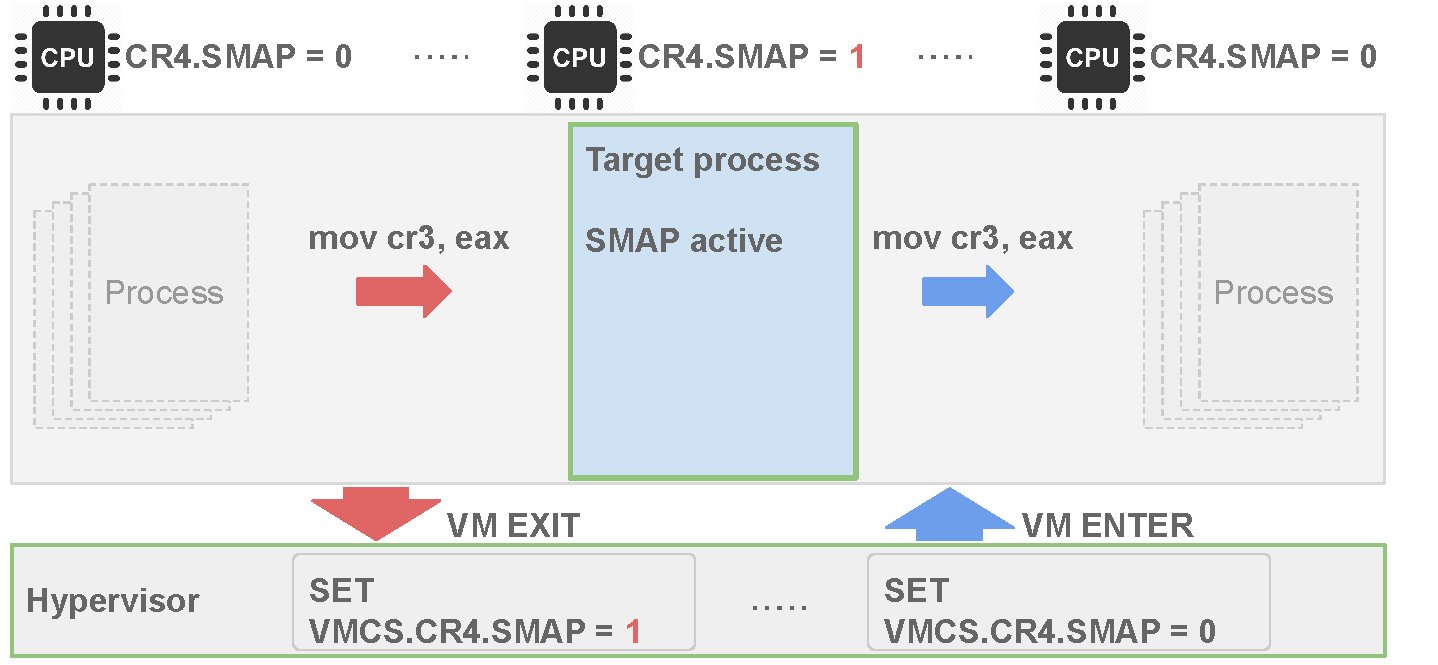
\includegraphics[width=0.47\textwidth]{figures/processmap4}
  \centering
  \caption{Operations on the CR3 register are the decisive characteristic of process context switching, which triggers VM exit by default. By setting the SMAP bit in the CR4 image of the VMCS.GuestArea, it updates the CPU CR4 when the hypervisor enters the virtual machine again. Therefore, it is possible to use the hypervisor to enable the SMAP feature when a specific process is running on the CPU.}
  \label{fig:processmap}
\end{figure}


By monitoring the process context switch event, namely, operations on the CR3 register, the hypervisor can temporarily enable/disable SMAP to make it only effective in the context of specific processes. ~\autoref{fig:processmap} shows that \texttt{mov cr3, eax} triggers a VM exit event, and the hypervisor receives it. If the new CR3 belongs to one of the target processes, the hypervisor sets the CR4.SMAP in the Virtual Machine Control Structure (VMCS), which is the data structure that updates the real CPU registers when entering the virtual machine. After returning to the guest virtual machine, the SMAP is active. When this process switches out, the hypervisor again receives the event and unset CR4.SMAP. Therefore, this particular process has the illusion that SMAP is active in the system while other processes feel the opposite.


The hypervisor inevitably brings performance overhead. However, it makes the mitigation more configurable. Due to the nature of local privilege escalation attacks, system processes that already have high privilege are not threats. Therefore it is not very meaningful to protect them, which reduces the overall performance overhead.  Additionally, as previously mentioned, SMAP confinement is also necessary to prevent deadlock caused by nested SMAP exceptions. Therefore we consider the hypervisor framework as one contribution of this paper.

%! TEX root = 'main.tex'

%\section{Experiments}

\section{Implementation}
\label{sec:implementation}

This section provides the implementation details and discusses the issues that we encountered during the development.



\subsection{Page Faults}


Exception handling is the primary method of \name. We leverage \texttt{SMAP} exception to notify the kernel-to-userspace access and next use exception to solve the read and write conflicts. Those events are all categorized as page faults. A page fault is a type of exception raised by the CPU when accessing a virtual page. The page ``fault'' mostly is not an error. It is the CPU's mechanism to implement virtual memory. For example, a page absence page fault is recoverable once the system assigns the physical page back.

We need to handle page fault exceptions before the system does.
Because the page fault caused by \texttt{SMAP} is fatal. It is not recoverable by design. Additionally, the followed exceptions that are related to the protection should not handle by the system either. We must also be careful with the exception that should send to the system, such as page absence. Because if we accidentally process those, it may cause the system to malfunction. To identify the cause of a page fault is not easy.  When page fault happens, the CPU pushes a 32-bit error code into the kernel stack with the format shown in~\autoref{fig:pagefaulterrorcode}.  Unfortunately, there is no exact error code regarding \texttt{SMAP}.  Still we can decide from the values in the kernel stack such as \texttt{CS:EIP}, \texttt{SS:ESP}, \texttt{EFLAGS} and the value from \texttt{CR2} and \texttt{CR3}.

\begin{figure}[th]
  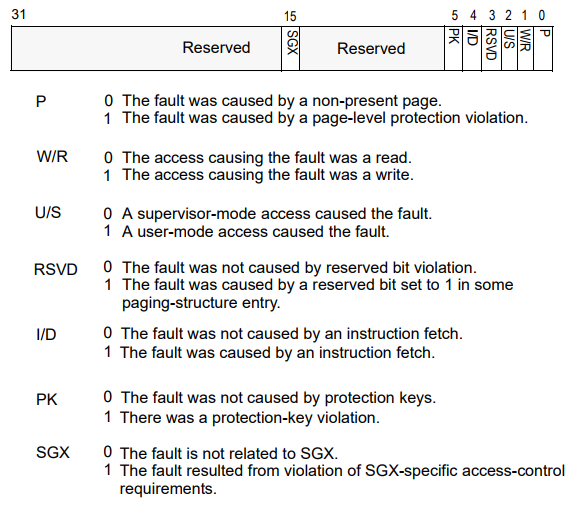
\includegraphics[width=0.47\textwidth]{figures/pagefaulterrorcode}
  \centering
  \caption{Page Fault Error Code.~\cite{intelinterrupt} Notice, there is no exact error code regarding \texttt{SMAP}. In the context of an \texttt{SMAP} exception, the \texttt{U/S} bit is zero, which indicates kernel-mode access. We still need to combine this information with the faulting address and \texttt{CS} segment register to confirm the cause.}
  \label{fig:pagefaulterrorcode}
\end{figure}



We need to filter out the irrelevant exceptions first. For example, \texttt{P:0} in the error code indicates the page absence, and we must pass it to the original page fault handler without any modification. We have not observed a \texttt{SMAP} exception on the invalid page, even though the error code may have combined bits. Other than that, \texttt{U/S:1} shows it is user-mode access, which will not cause \texttt{SMAP} exception.  The \texttt{Current Privilege Level (CPL)} in the \texttt{cs} segment register also reveals the context. Additionally, we keep track of the protected or relevant pages, which helps to identify the exceptions.



After filtering, ~\autoref{algo:pagefaulthandler} shows the basic algorithm to handle the \texttt{SMAP} and related exceptions.


\begin{algorithm}[ht]
\begin{algorithmic}[1]
\small
\Procedure{PageFaultHandler}{}

\State $address\gets cr2$ 
\State $pte\gets \Call{\textbf{GetPte}}{address}$
\State $teb\gets fs:0x18$

\If{SmapViolation}
	\State $pages[]\gets \Call{\textbf{AddPage}}{$address, pte, cr3, teb$}$
    	\State \Call{\textbf{SetPageKernel}}{pte}
    	\State \Call{\textbf{FlashTlb}}{address}
    	\State \Return{Re-execute}
\ElsIf{UserAccessProtectedPage}
	\If{error.WRITE}
    		\Repeat 
		\State \Call{\textbf{Sleep}}{}
        		\If{\Call{\textbf{CheckPtePermits}}{pte}}
        			\State \Return{Re-execute}
        		\EndIf
        	\Until{$count < 10$}
        	\State \Return{TerminateThread}
	\Else
    		\State \Call{\textbf{SetPgeUserReadonly}}{pte}
    		\State \Call{\textbf{FlashTlb}}{address}
        	\State \Return{Re-execute}
	\EndIf

%%\ElsIf{$user\_write\_readonlypage$}
%%	\If{\Call{HAS\_RECORD}{pte}}
%%    \EndIf

\EndIf
\State \Return{OriginalHandler}
   
\EndProcedure
\end{algorithmic}
\normalsize
\caption{Page Fault Handler}
\label{algo:pagefaulthandler}
\end{algorithm}



\textbf{\textit{Enable Interrut.}} The page fault exception is called through an \texttt{Interrupt Gate}~\cite{intelinterrupt}. Therefore, when entering the page fault handler, the CPU clears \texttt{EFLAGS:IF} automatically prevents subsequent interrupts from interfering with the handler's execution. Since we need to walk through the page table, it may access an invalid page, which triggers a nested page fault exception to bring the page back from disk. Therefore we need to set \texttt{EFLAGS:IF} before the page table walk.

\subsection{Hypervisor}

% moved to background
%Intel \texttt{Virtual-Machine Extensions (VMX)} provides hardware-assistant virtualization, which adds 13 new instructions: \texttt{VMPTRLD}, \texttt{VMPTRST}, \texttt{VMCLEAR}, \texttt{VMREAD}, \texttt{VMWRITE}, \texttt{VMCALL}, \texttt{VMLAUNCH}, \texttt{VMRESUME}, \texttt{VMXOFF}, \texttt{VMXON}, \texttt{INVEPT}, \texttt{INVVPID}, and \texttt{VMFUNC}. \texttt{VMX} supports two modes, namely root and non-root mode, where in root mode runs the hypervisor, and virtual machines or called guest runs in non-root mode. On x86 architecture, the CPU has 4 protection rings, where the kernel runs at \texttt{ring 0}, the highest priority ring, and the user programs runs at \texttt{ring 3}, while the other two rings are not used. With VMX, the root model is often viewed as the \texttt{ring -1}. \texttt{VMXON}/\texttt{VMXOFF} enters/exits \texttt{VMX} mode. The \texttt{Virtual Machine Control Structure (VMCS)} is the most important data structure, which stores the data and state of one virtual CPU for one virtual machine. Each core in a physical CPU has a \texttt{VMCS} pointer. It points to the physical address of one \texttt{VMCS}. \texttt{VMPTRLD} loads the \texttt{VMCS} pointer from physical memory and makes it active and current. On contrary, \texttt{VMCLEAR} stores \texttt{VMCS} active states back to memory and makes it inactive. Although hypservisor fully aware the physical address of each \texttt{VMCS} but it can not modify them directly. All the operationgs on \texttt{VMCS} should go through instruction \texttt{VMREAD} and \texttt{VMWRITE}.



We do not use a bare-metal hypervisor because we create only one virtual machine, the current system, and do not need to emulate hardware. We use multiple \texttt{VMCS} that each represent one logical processor of the physical CPU and loads the logical processor's run-time state. Essentially, each processor exists in the system has its \texttt{VMCS}, hence no need to reload \texttt{VMCS} pointers.

%The \texttt{VMCS} contains many data-fields that are related to aspects of a virtual machine. They are organized into six logical groups, namely, \texttt{Guest-state area}, \texttt{Host-state area}, \texttt{VM-execution control fields}, \texttt{VM-exit control fields}, \texttt{VM-entry control fields}, and \texttt{VM-exit information fields}. The last four groups compose \texttt{VMX controls}, which control the virtual machine's behavior such as when to exit to the hypervisor. In \texttt{VMX}'s term, \texttt{VM entry} is the transition into the \texttt{VMX} non-root operation while \texttt{VM exit} is the transition from the \texttt{VMX} non-root virtual machine to the VMX root  hypervisor. When VM exit, the processor stores its state into the \texttt{Guest-state area} and loads \texttt{Host-state area} into hardware. In contrast, it loads \texttt{Guest-state area} and stores \texttt{Host-state area} when entering the virtual machine. For our run-time load hypervisor, we set up those two areas mostly identical to the current CPU state but with different entry addresses, which, in root mode, serves the VM exit event handler's purpose. With that, we call \texttt{VMLAUNCH} respectively on each processor to enter the virtual machine. We control when the virtual machine exit through \texttt{VMX control} settings. 

To monitor the process context switch, we need the virtual machine exit on control register operations. In the event handler, the hypervisor can modify CPU state through \texttt{Guest-state area}, in this case, it is \texttt{CR4.SMAP}. After that, the hypervisor invokes \texttt{VMRESUME} to re-enter the virtual machine.

\subsection{Updating PTE}

We modify the bits in \texttt{PTE} to change a page's attribute. Updating system metadata such as the page table needs synchronization with other system components. Typically, the modifier should hold a global lock first. However, as a third-party kernel module, we do not have such information on Windows internal data.


%%\begin{lstlisting}[style=code, float]
%\begin{lstlisting}[style=code] 
%typedef struct _PTE_HARDWARE
%{
%	ULONG Valid : 1;
%	ULONG Write : 1;
%	ULONG Owner : 1;
%	ULONG WriteThrough : 1;
%	ULONG CacheDisable : 1;
%	ULONG Accessed : 1;
%	ULONG Dirty : 1;
%	ULONG Reserved : 1;
%	ULONG Global : 1;
%	ULONG Ignored: 3;
%	ULONG PageFrameNumber : 20;
%} PTE_HARDWARE, *PPTE_HARDWARE;
%
%typedef struct _PTE {
%	union {
%		ULONG Long;
%		PTE_HARDWARE Hard;
%	} u;
%} PTE, *PPTE;
%\end{lstlisting}

\begin{figure}[th]
  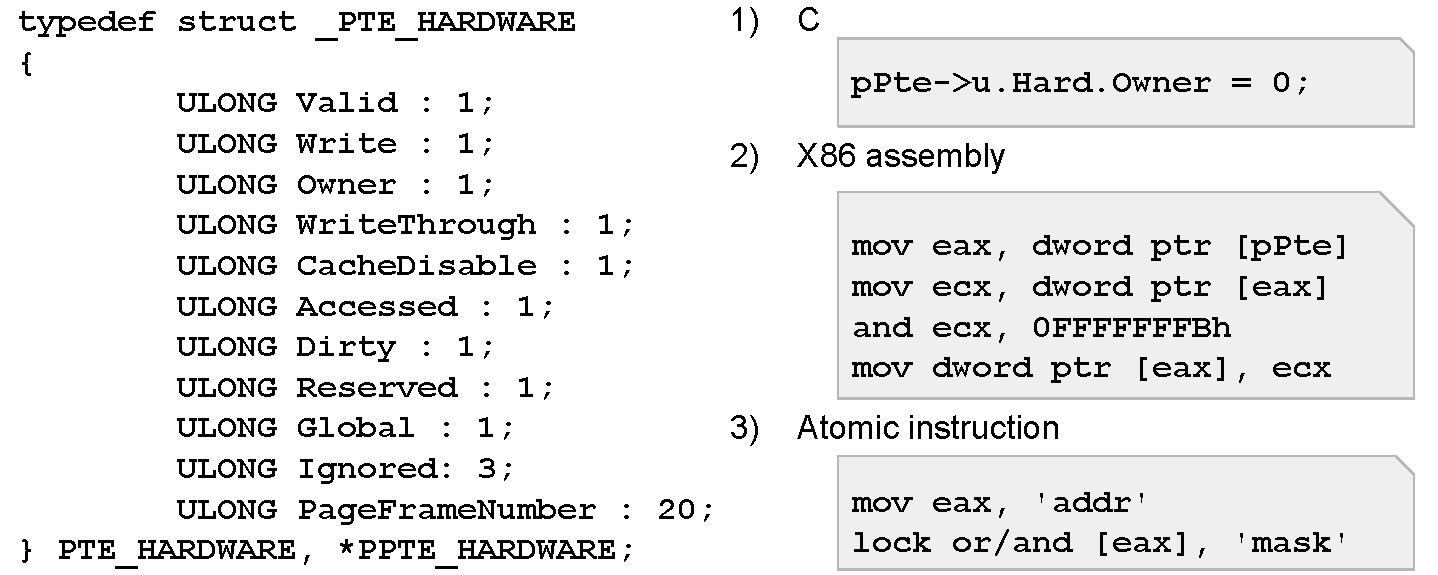
\includegraphics[width=0.47\textwidth]{figures/ptestructcode}
  \centering
  \caption{Left: PTE structure defined in C. Right: C code for changing one bit in the PTE structure, the corresponding assembly code generated by Microsoft C/C++ compiler, and the atomic instructions that serve the same purpose.}
  \label{fig:ptestruct}
\end{figure}


In a typical kernel-level TOCTOU attacking scenario, the attacker races with the kernel at full speed, so will our mitigation triggered. We modify the page table rapidly. Hence we need to make our operation as atomic as possible. ~\autoref{fig:ptestruct} shows the \texttt{PTE} data structure defined in C on a 32-bit system. The C code at \texttt{\textcircled{1}} changes the \texttt{Owner} a.k.a \texttt{U/S} bit to zero, which makes it a kernel-mode page. \texttt{\textcircled{2}} is the assembly code generated by a compiler, where once C statement needs three assembly instructions. However, during the three instructions, the current thread may be interrupted, or other threads may also update the same \texttt{PTE} due to the race condition, which occurs multiple times when we test the exploit agast \name. We use the locked atomic instruction~\cite{intelmanualchapter8} instead of the compiler-generated assembly code, as shown at \texttt{\textcircled{3}}. It guarantees that the update on one \texttt{PTE} is intact. 

In the future, if the operating system takes such mitigation into its source tree, it will solve such a synchronization issue entirely.

\subsection{TLB Flushing}
%A translation lookaside buffer(TLB), as mentioned earlier, is a memory cache that is used to store the mappings between virtual pages and physical pages. Different than data cache, TLB is not entirely transparent to the operating system. When operating system updates page tables, corresponding TLB entries need to be invalidated.
%
%Instruction "INVLPG" is used to invalidate a TLB entry. It has a source operand which is a virtual memory address. "INVLPG" only invalidate TLB entries on the current CPU, so on multiple processor system, we need to execute it on every processor that has the same TLB entry. To do do, we need to issue an inter-processor interruption(IPI) to inform all the CPU cores in the system.
%
%IPI allows a processor to send interrupt signals to other processors. It's different than normal "interrupt" which go through an IRQ line. IPI signal needs to be sent via the advanced programmable interrupt controller(APIC) bus which connects all the local APIC of every CPU core.
%
%In our implementation, we actually reuse some of the functionality from Windows operating system to issue the IPI for TLB flushing. Because Windows' MMU also need the same function to flush TLB, we found the address of the related internal functions at run-time, call it when we update a PTE. 
%



When we apply our mitigation on real hardware instead of a virtual machine, one crucial issue is the need to flush the TLB.  Translation Lookaside Buffer (TLB) is a memory cache used to reduce the time taken to access a virtual memory location. It stores the recent translations of virtual memory to physical memory. Different than data cache, TLB is not entirely transparent to the operating system. When the operating system updates a page table entry, the corresponding TLB entry needs to be invalidated.

Instruction INVLPG invalidates a TLB entry. It only has a source operand, which is a virtual memory address. INVLPG only affects the current CPU. However, on a multiple processor system, each processor core has its TLB. Therefore we need to do this on every core. For this purpose, we need to issue intel-processor interruption (IPI) to each core through APIC. Symmetric multiprocessing (SMP) system uses IPI messages to distribute interrupts among the processors in the system or execute system-wide functions such as booting up processors or distributing work among a group of processors. 

In this project, we find a Windows kernel internal function, KeFlushSingleTb(). It sends IPI to all processors to invalid a particular TLB entry, as mentioned above. The hardware abstraction layer (HAL) eventually sends the IPI, so the kernel does not need to mind the actual hardware differences.


\subsection{Crashing a Faulty Thread}

As mentioned earlier, to solve the problem that a user thread tries to write a protected page, instead of crashing the thread immediately, our approach is to hold the thread for some milliseconds, waiting for the function to end. To avoid any deadlock or blockage caused by a faulty program, we only allow for several retries. 

Since it is troublesome to call a series of undocumented functions to handle exceptions. We choose to let the operating system terminating it. We clears ``p'' bit of the corresponding PTE as well as changing the error code to a value that indicates ``accessing an invalid page'' instead of ``writing an read-only page''. Because we can't synchronize with MMU, when we passing the exception to the original page fault handler, the PTE's attributes could be changed within the short period of time due to another SMAP exception, this could happen especially in the attacking scenario. 

%global hook, it may use shared memory,  before put it here, probably should figure out how page permits works on shared page


\subsection{Special Cases}
We assume 32bit Windows operating system use the default 2G/2G user/kernel split where user space is below 0x7FFFFFFF. More precisely, a kernel variable MmUserProbeAddress contains the highest possible address for user data, which is set to 0x7FFF0000. And we learn that one page locates at 0x7FFE0000 is defined as \texttt{USER\_SHARED\_DATA}. It's a shared page between user mode and kernel mode, meaning the same physical page is mapped both at 0x7FFE0000 and 0xFFDF0000. It's a read-only page and contains a lot of process settings such as system time. Kernel needs to read this page a lot. We treat such page specially to improve performance. 



%! TEX root = 'main.tex'

\section{Evaluation}
\label{sec:ktoctou-evaluation}

In this section, we evaluate \name's performance overhead and how it protects the operating system from real-world vulnerabilities.


\subsection{Performance}
In this section, we focus on performance evaluation.
As previously mentioned, \name has two key components, the system module and the hypervisor. To present the performance impact introduced by this mitigation, we conduct the tests in three parts. 

All tests run on the PC with Intel Core I5-6400 (6 GEN CPU Skylake), ASUS H110M-C motherboard (Intel H110 Chipset, Realtek RTL8111H Network Controller), 8GB RAM, and 500GB hard disk.

\textbf{textit{Benchmarks.}} The hypervisor plays an essential part in \name. Without the hypervisor confining the SMAP feature, it would not be possible to debug a complex system like Windows with a system-wide unsupported feature. Nowadays, a hypervisor is part of the cloud computing infrastructure and can be regarded as a built-in component. The Windows 10 operating system even brings its native hypervisor to deliver security goals. Under those circumstances, \name can be added to the existing hypervisor with less performance overhead imposed on the system. 

To evaluate the hypervisor's performance overhead, we use the well-known benchmark SPEC 2006. We understand that this benchmark is for processor instruction evaluation, specifically for microarchitectural aspects, such as instruction execution, branch prediction accuracy, cache policies. We choose several programs from the set. They are all non-GUI and computational intensive programs. Therefore the performance overhead incurred is primarily due to the hypervisor. Although our hypervisor and Windows HVCI have different objectives, we compare them to show that run-time protection utilizes virtualization techniques is practical.

\begin{figure}[th]
  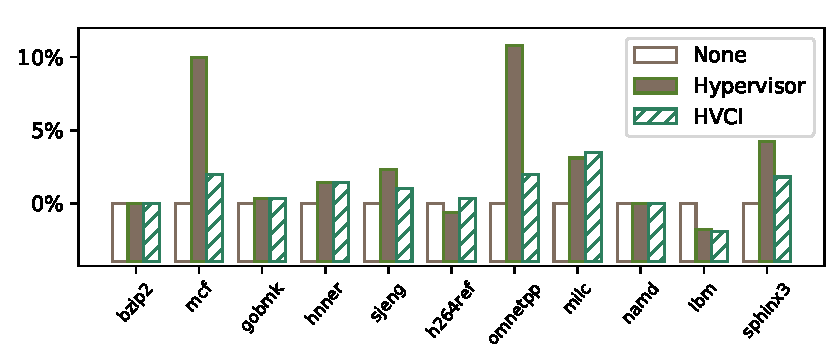
\includegraphics[width=0.47\textwidth]{figures/benchmark3}
  \centering
  \caption{Performance overhead on the SPEC benchmarks incurred by the run-time load hypervisor. HVCI represent the Windows 10 native hypervisor for Hypervisor-Protected Code Integrity. All overheads are normalized to the unprotected system running benchmark.}
  \label{fig:ktoctou-benchmark}
\end{figure}


\autoref{fig:ktoctou-benchmark} shows that hypervisor's performance overhead is acceptable, on average, 3.25\%. HVCI yields a modest performance overhead of 0.81\%.

% show my respect.. maybe remove it later

Our hypervisor is slower than HVCI, particularly in two benchmark programs. Learning more about computer architecture and virtualization techniques, we wish to improve our hypervisor to perform better.



\textbf{\textit{Non-trivial Applications.}} We also evaluate \name on several non-trivial applications, as shown in~\autoref{fig:ktoctou-performance}. The applications we choose are meaningful because the kernel-TOCTOU vulnerability may threaten them. For example, a web server such as Nginx normally runs in a non-root account and takes external requests. 

To test web servers, we count their response time for a web request. For compression software, the test is to compress large files. We also use speedtest1.c, which is a performance testing program for sqlite3. The result shows that the performance overhead is acceptable. 

\begin{figure}[th]
  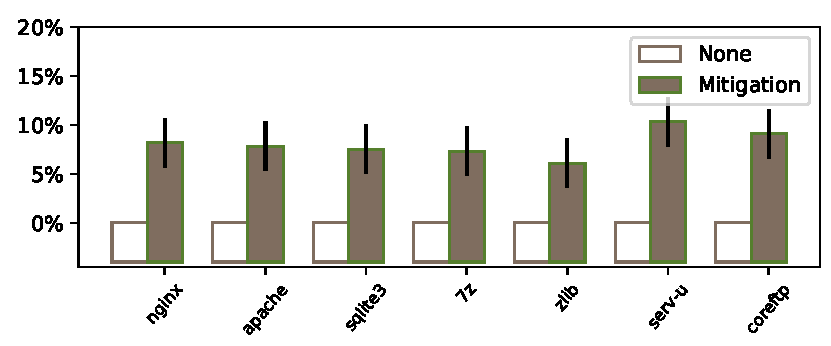
\includegraphics[width=0.47\textwidth]{figures/performance4}
  \centering
  \caption{Performance overhead in non-trivial applications. Overhead mostly being introduced on system calls that need to fetch user parameters}
  \label{fig:ktoctou-performance}
\end{figure}





\textbf{\textit{GUI.}} Through our investigation, we find that the Windows graphical subsystem, namely, Win32k.sys, has the most double-fetch issues.  Because GUI programs need to redraw their graphical components frequently, they invoke the win32k system calls a lot, even for a simple program such as Windows notepad. Therefore,  our mitigation incurs an unneglectable performance over GUI programs. The overhead is primarily affected by how often the interface is refreshed. For example, if minimizing a GUI program's window, its performance will not be slow down by the graphical interface at all. We compare GUI programs with non-GUI programs in the following aspects: the number of user pages accessed by kernel per system call and how many double fetches occur. We drag the GUI program's window to trigger redraw, and we send one URL request to the web servers per second. The measurement takes the first 500 system calls.

\begin{center}
\begin{table}[ht]
	\small
	%\renewcommand{\arraystretch}{1.3}
	\caption{System call count and user-pages accessed for GUI \& non-GUI programs }
	\label{table:pages}
	\centering
%	\begin{tabular}{ l|p{0.04\textwidth}|p{0.108\textwidth}|l|p{0.045\textwidth}|p{0.045\textwidth} } 
%	\begin{tabular}{ c@{}|@{}c@{}|@{}c@{}|@{}c@{}|@{}c@{}|@{}c }   
	\begin{tabular}{@{}>{\centering\arraybackslash}m{1.40cm}@{}|
			@{}>{\centering\arraybackslash}m{1.15cm}@{}|
			@{}>{\centering\arraybackslash}m{2.30cm}@{}|
			c|
			@{}>{\centering\arraybackslash}m{1.15cm}@{}|
			@{}>{\centering\arraybackslash}m{0.97cm}@{} } 
		\hline
		Programs & System Calls & Protected Pages(r, w) & \textbf{avg.} & Double Fetch & Time (ms)\\ 
		\hline
		nginx & 500 & 711(711, \textbf{0}) & 1.42 & \textbf{223} &12312\\ 
		apache & 500 & 689(689, \textbf{0})  & 1.38 & \textbf{205} &11339\\ 
		notepad & 500 & 1434(1102, 241) & 2.87 & \textbf{1373} & 1859 \\ 
		freecell & 500 & 1352(1165, 187) & 2.70 & \textbf{1266} & 1500 \\ 
		\hline
	\end{tabular}
\end{table}
\end{center}


\autoref{table:pages} shows some interesting results. Refreshing the GUI takes tremendous system calls. As expected, both the kernel and the Win32k subsystem accesses user pages, but the win32k accesses more than the kernel. They both \textit{capture} the user parameters at each system call, but the win32k module read/write more user data even in the middle of a system call.


We also count the number of reads and writes on user pages. For non-GUI programs, the number of writes is zero, which is strange because most system calls need to write results back to the user program. With investigation, the causes are as follows. Windows provides three methods to transfer data between system calls and user programs, namely, Buffered I/O, Direct I/O, and Neither Buffered Nor Direct I/O. Among the three, the kernel mostly uses Buffer I/O and Direct I/O, which do not need to write to user-mode buffer directly. However, the kernel still needs to write user-mode variable such as the filehandle in system call \texttt{NtCreateFile}.
~\autoref{fig:probecode} shows the pseudo-code similar to what the kernel uses to validate user parameters. We can see that the code always reads the variable first and the SMAP exception only captures first access. Therefore, this coding style is another cause for the zero writes. The results show the kernel is well regulated on accessing user data. On the other side, the Win32k module has many writes, which tell a different story.


\begin{figure}[th]
  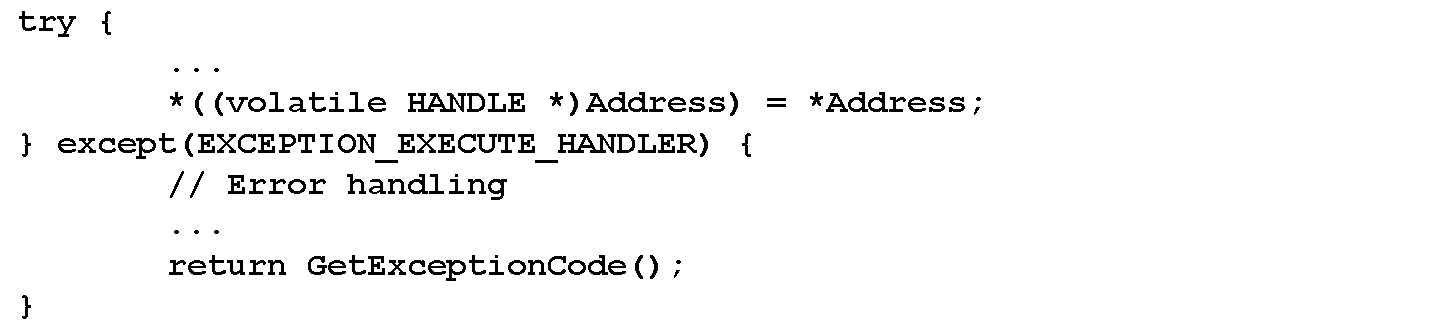
\includegraphics[width=0.47\textwidth]{figures/probecode}
  \centering
  \caption{Pseudo-code for validating a file handler.}
  \label{fig:probecode}
\end{figure}



% for later reference
%Buffered I/O
%The operating system creates a nonpaged system buffer, equal in size to the application's buffer. The I/O manager copies user data into the system buffer for write operations before calling the driver stack. For read operations, the I/O manager copies data from the system buffer into the application's buffer after the driver stack completes the requested operation.
%
%Direct I/O
%The operating system locks the application's buffer in memory. It then creates a memory descriptor list (MDL) that identifies the locked memory pages and passes the MDL to the driver stack. Drivers access the locked pages through the MDL.
%
%Neither Buffered Nor Direct I/O
%The operating system passes the application buffer's virtual starting address and size to the driver stack. The buffer is only accessible from drivers that execute in the application's thread context.
%




The column \textit{Double Fetch} shows the user-addresses that are read more than once during individual system calls. We trace this information with the fuzzing tool as previously introduced in~\autoref{sec:ktoctou-experiment}. Many of those double-fetch records are duplicates and benign. The kernel needs to read data from Process Environment Block (PEB) or Thread Environment Block (TEB), data structures located in userspace.  However, the Win32k module has many more cases. ~\autoref{table:doubleread} gives a glimpse of them. Every two rows indicate a double-fetch case, where after the first read, the subsequent instruction revisits the same address shortly after, and the identical CR3 and TEB show that two fetches are from the same thread of the same process.

Furthermore, with reverse-engineering effort, we find that the Win32k module directly read the user variable and without the protection of a try-catch block in some of those cases. It is dangerous. The user programs can free the user memory and cause the kernel code to access an invalid page without protection, which leads to a crash.

\begin{center}
	\begin{table}[ht]
		\small
		%\renewcommand{\arraystretch}{1.2}
		\caption{In the selected double-fetch results, for every two lines, they have the same CR3 and TEB, which indicate the two records are from the same process, same thread. The two EIP are shortly apart, but the addresses they reference are the same and from userspace.}
		\label{table:doubleread}
		\centering
		%\begin{tabular}{ l l l l }
		\begin{tabular}{@{}>{\centering\arraybackslash}m{2.05cm}@{}|
				@{}>{\centering\arraybackslash}m{2.05cm}@{}|
				@{}>{\centering\arraybackslash}m{2.05cm}@{}|
				@{}>{\centering\arraybackslash}m{2.05cm}@{} } 
			\hline
			Cr3 & Eip & Addr. & Teb \\
			\hline
			0x6d40320 & 0xbf812de4 & \textbf{0x4808c4} & 0x7ffdd000 \\
			0x6d40320 & 0xbf812e4b & \textbf{0x4808c4} & 0x7ffdd000 \\
			\hline
			0x6d40320 & 0xbf812dea & \textbf{0x4808c8} & 0x7ffdd000 \\
			0x6d40320 & 0xbf812e55 & \textbf{0x4808c8} & 0x7ffdd000 \\
			\hline
			0x6d40320 & 0xbf812daf & \textbf{0x480750} & 0x7ffdd000 \\
			0x6d40320 & 0xbf812e21 & \textbf{0x480750} & 0x7ffdd000 \\
			\hline
			0x6d40320 & 0xbf80c04d & 0x7ffdd206 & 0x7ffdd000 \\
			0x6d40320 & 0xbf812ebe & 0x7ffdd206 & 0x7ffdd000 \\
			\hline
		\end{tabular}
	\end{table}
\end{center}



%Part of the overhead is introduced due to the overall intercepting of page fault exceptions of the system. The page fault handler is called in high frequency. Our page fault hook currently is installed directly in the IDT table of each processor. Hence every page fault exception goes through our handler. Even though, in the very begining, we pass through exceptions that doesn't belong to the target process, still extra instructions are executed for each exception.

%Although we use virtualization techniques, but the hypervisor we use is a very simple one. Unlike commercial virtualization solutions such as VMWare, Xen and Qemu+Kvm, ours doesn't emulate any hardware devices nor intercept further page mapping translate that between host and guest. Only several types of VM-Exit is inevitable such as control register accessing which we do need to handle it too.

Considering the kernel is fully aware of the untrustworthy user-supplied parameters, we believe it is practical to eliminate the SMAP exceptions during parameter validating. It will promote the performance of mitigation. As was done with the Linux kernel, the SMAP feature is temporarily disabled during \texttt{copy\_from\_user()} and \texttt{copy\_to\_user()}, the gateways. In Windows kernel, ProbeForRead() and ProbeForWrite() are the equivalent of that. However, such "Probe" has many variants. For example, ProbeAndWriteHandle(), ProbeForWriteIoStatus(). Some of them are macros instead of functions, making it difficult to change all of them without recompiling the kernel. On the contrary, the code piece that uses user variable is spreading across the module. The repairing process will take great effort. 

\subsection{Case Study}

%We test it on the Windows XP sp3 system with the vulnerable win32k.sys file whose version is 5.1.2600.5512. Because SMAP only available at Intel 5th generation CPU (architecture code name Broadwell). Hard-disk controller which integrated in the CPU corresponded chipset doesn't support ATA mode anymore, and Windows XP system doesn't support AHCI mode, so it's difficult to install it on a modern PC. Our testing environment is established using a virtual machine. Particularly, VMWare Workstation 14 Player, emulated "Intel Core i5-6200U CPU (2 cores) with 1GB of RAM", option "Virtualize Intel VT-x/EPT or AMD-v/RVI" also enabled.

\textbf{\textit{CVE-2008-2252}} is a bug reported by Thomas Garnier in 2008 and fixed by Microsoft as part of the MS08-061 security bulletin.  It is a typical TOCTOU vulnerability addressed in many previous research works~\cite{serna2008ms08}~\cite{wang2019dftracker}~\cite{jurczyk2013identifying}. To evaluate the effectiveness of our mitigation, we want to test it on a real hardware machine. SMAP and SMEP are only available on a relatively new processor, Intel 5 generation CPU (architecture code name Broadwell). It is troublesome to install the Windows XP operating system on a modern PC. The chipset with an integrated hard disk controller no longer supports IDE mode, and Windows XP does not support the advanced host controller interface (AHCI) either. For us, we need an additional AHCI driver for Windows XP and a tool to virtualize a floppy drive~\cite{installxpskylake} to provide it during the installation.

We write a proof-of-concept (POC) program to exploit the CVE-2008-2252 vulnerability. If it flips the user-mode variable between the two kernel fetches, it will create a memory buffer overflow in the kernel. We test it against our mitigation in a multi-processor system.



The exploit creates two threads. One thread first allocates a virtual page at address 0 then use it as the parameter for the vulnerable system call. Using page zero is a necessity to bypass the sanity check of the system call NtUserMessageCall(). Then, it repeatedly calls the upper layer vulnerable Win32 API \texttt{SendMessage()} (\texttt{WM\_COPYDATA}) with the malicious parameters. \texttt{SendMessage()} calls a lower layer function \texttt{NtUserMessageCall()}, which eventually calls the vulnerable win32k internal function \texttt{xxxInterSendMsgEx()}. The other thread keeps flipping the key variable on page zero simultaneously.

\begin{figure}[th]
  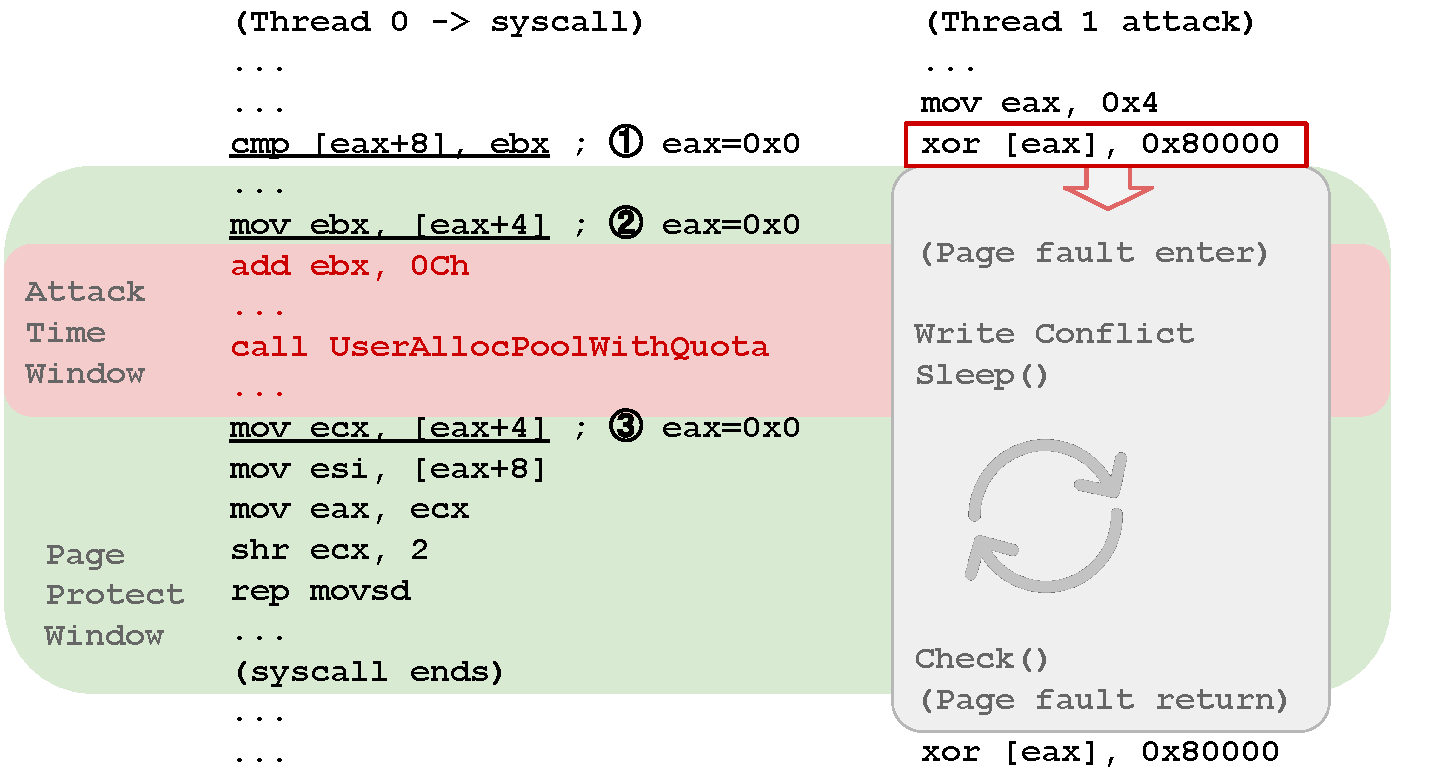
\includegraphics[width=0.47\textwidth]{figures/ms08061case2}
  \centering
  \caption{The attack thread tries to flip the data within the attack window, between instruction \texttt{\textcircled{2}} and \texttt{\textcircled{3}}. The kernel first touches the page at instruction \texttt{\textcircled{1}}, then the mitigation protects it afterward until the end of the current system call, creating the larger page-protect-window. As soon as the attack thread writes the protected page, the page fault handler suspends it until the protection ends.}
  \label{fig:ms08061case}
\end{figure}

%In the attack, as shown in ~\autoref{fig:ms08061case}, the \textcircled{2} and \texttt{\textcircled{3}} are the places where vulnerable user-mode variable pcbData are referenced, it's address is 0x4. But the first time the zero page get accessed is \textcircled{1} where several instruction ahead of \textcircled{2}, it triggers an page fault exception (cased by SMAP). Therefore this page will be marked as a kernel page by our page fault handler. From this moment until the end of the current system call, this page will be protected from modifying by either as a kernel page or a user page with read-only permit. If the attacking thread try to modified it, another page fault exception  will be raised because of access violation. Then the attacking thread will be held for 30 milliseconds before it try to re-execute the faulting instruction again, for as many as 10 times. If not possible, the attacking thread will be terminated. We can see that during the protection, memory reads at \textcircled{2} and \textcircled{3} are kept consistent.

As shown in~\autoref{fig:ms08061case}, the kernel reads the user-mode variable at address 0x4 twice at \texttt{\textcircled{2}} and \texttt{\textcircled{3}}. Any data changes during this time will cause data inconsistency in the kernel. Therefore it is the time window for the attack. The attack thread tries to enlarge the value read at \texttt{\textcircled{3}}. Our protection needs to cover the entire attack time window so that the attack thread can not change the user-mode variable during it. In this case, at \texttt{\textcircled{1}}, several instructions before \texttt{\textcircled{3}}, the CMP instruction operating on page zero, causes a SMAP exception. Our page fault handler sets page zero to kernel-mode until the current system call, that is, NtUserMessageCall(), ends. This period covers the entire attack time window. Once the attack thread tries to write the protected page, it will raise a page fault exception, and our page fault handler will suspend the current thread, waiting for the release of the page.


%\textbf{\textit{CVE-2013-1254}} is another typical TOCTOU vulnerability that found in Windows win32k module~\cite{jurczyk2013identifying}. It effects both Windows XP and Windows 7. 

%A series of same kind of vulnerability found in 26 functions of module win32k.


CVE-2013-1254. Similar to the one above mentioned, CVE-2013-1254 is another typical TOCTOU vulnerability. It is a family of 27 distinct vulnerabilities~\cite{ms13016}~\cite{jurczyk2013identifying} in the win32k module. It affects a variety of operating systems from Windows XP to Windows Server 2012.

%\begin{lstlisting}[style=code] 
%.text:BF8A993F   mov   eax, _W32UserProbeAddr
%                       .
%                       .
%.text:BF8A9973   @cmp   [ecx+8], eax@    
%.text:BF8A9976   jnb   short loc_BF8A997B
%.text:BF8A9978   @mov   eax, [ecx+8]@    
%.text:BF8A997B
%.text:BF8A997B loc_BF8A997B:                           
%.text:BF8A997B   mov   ecx, [eax]
%.text:BF8A997D   mov   eax, [eax+4]
%\end{lstlisting}
%%\captionof{lstlisting}{Flawed code in win32k.sys function SfnINOUTSTYLECHANGE()}

\begin{figure}[th]
  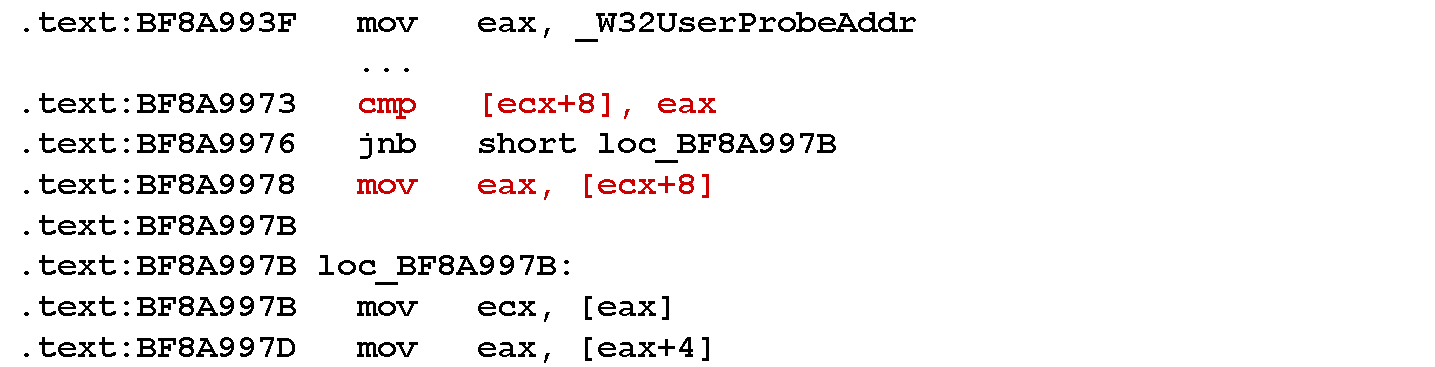
\includegraphics[width=0.47\textwidth]{figures/cve-2013-1254}
  \centering
  \caption{The family of the 27 vulnerabilities in the win32k module is mostly around the parameter sanity check. The checking code with \texttt{\_W32UserProbeAddress} makes sure that the parameters passed in reside in userspace. It is a classic time-to-check-to-time-to-use. When checking, the \texttt{[exc+8]} is less than \texttt{\_W32UserProbeAddress}, when using, it could change to a kernel address by another user-mode thread. Furthermore, the malicious address that passed the sanity check may point to an essential kernel data structure, hence gives the attacker kernel write capability.}
  \label{fig:cve-2013-1254}
\end{figure}




They have the same patterns. The code is mostly around the \texttt{\_W32UserProbeAddress}, which is a value that indicates the highest possible address for user-mode variables. As shown in~\autoref{fig:cve-2013-1254}, the flawed code in red first gets the value from \texttt{ecx+8} and compare it with \texttt{\_W32UserProbeAddress}. Afterward, it gets the data again to eax, which is the second fetch. The attacker can abuse this, changing the value to bypass the parameter sanity check, for example, send in a kernel-mode address. 


Therefore, when the instruction \texttt{cmp [ecx+8]}, eax triggers the SMAP exception, our mitigation protects this page until the current system call ends.



\section{Discussion}
\label{sec:ktoctou-discussion}


\textbf{\textit{Fuzzing.}} \autoref{sec:ktoctou-experiment} presents new method of fuzzing kernel TOCTOU vulnerabilities. A practical alternative is to utilize hardware data breakpoints. Data breakpoint~\cite{krishnan2009hardware} a.k.a watchpoint is a debug feature.  It raises debug exceptions when accessing the set memory locations.  DataCollider~\cite{krishnan2009hardware} use it to dynamically detects data races in kernel modules. Through static analysis,  DataCollider first decides the sampling set. Then it inserts code breakpoints, and when one code breakpoint fires, it uses a data breakpoint to trap the second access to detect conflicts. Although only four data breakpoints are available on each processor core, it is sufficient for hunting data race bugs.


Qemu~\cite{bellard2005qemu} with the dynamic binary translation (DBT)~\cite{ebcioglu2001dynamic} engine is a unique approach for fuzzing. It fully perceives the details of every instruction emulated, and it is fast enough to run comprehensive tests on the latest operating system. Its dynamic translation backend is called the tiny code generator (TCG)~\cite{bellard2009tiny} that converts binary code from the guest processor architecture to the host architecture. For example, it can take x86 guest code and turn it into an equivalent sequence of instructions natively executable on an ARM host. It also can add instrumentation code~\cite{quynh2015unicorn}. QEMU with TCG is still slower than the hardware assistant virtualization, but it runs much faster than Bochs, making it capable of more in-depth fuzzing.

%There is another proposal. First load a driver which sets up VM environment, puts OS run as a virtual machine, just like our project does. Then transfer into kernel mode, invalidate all user-mode data pages, for example, clear the “Present” flag for all top-level user-mode data page table entries. In such way that all kernel-mode access to 00000000-7fffffff yield a page fault exception. The hypervisor intercepts the page fault and set TF (Single Step) flag and restore the faulting page to let the OS successfully execute the faulting instruction. After that it intercepts DB exception and set the page back to invalidate.  But the drawback is also obvious, both the kernel and user mode will trigger the page faults exceptions, so in a multi-thread process, once one thread call into kernel mode, other user mode thread may be interrupted too often due to their data accessing.




\textbf{\textit{Write Conflicts.}} As previously mentioned in~\autoref{sec:ktoctou-design}, we solve the write conflicts by making the thread suspending inside the page fault handler until the current system call ends. We also considered other methods to solve this issue, such as a thread-level copy-on-write (COW) mechanism. When there is a write conflict, the page table splits, and the protected page has two different mappings in each so that the kernel and the user thread have their copy. Therefore, the user thread can freely write it without affects the kernel. The hypervisor maintains the newly forked page table and only use it to replace the CR3 when this particular thread is running. We use similar techniques for controlling the thread context switching~\cite{pan2017digtool}. Other than the CR3 operation,  we can monitor certain kernel data structures instead.  However, the issue lies in determining the time to merge the page tables and deciding which copy to take when there are data conflicts. Because even at the end of the current system call, many places on the page may change. Without the precise timing sequence information, it is hard to decide whether they would cause kernel-level TOCTOU issues and which copy has the latest data.



\textbf{\textit{Potential Attacks.}} When we discuss our mitigation with other security researchers, one researcher brought up a scenario as follows. Our mitigation protects a user page after the kernel access it. Although a user thread can not modify the page afterward, it can manipulate the kernel to do that. We acknowledged that this could be a possible attack because there are kernel vulnerabilities that give attacker kernel write capability. However, if the attacker already has such capabilities, the need to trigger another kernel-level TOCTOU vulnerability is questionable on a case-by-case basis.

\section{Related Work}
\label{sec:ktoctou-relatedwork}




%\textbf{Transactional Memory}~\cite{herlihy1993transactional}~\cite{shavit1997software}~\cite{rajwar2012intel}~\cite{haring2012ibm}~\cite{jacobi2012transactional}~\cite{click2009azul}~\cite{dice2009early} attempts to simplify concurrent programming by allowing memory read and write instructions to be executed in an atomic way. Usually memory access transactions are short-lived activities only when accessing a small memory area, such as a shared counter or shared double-linked list. Since transactional memory is limited resource, it's not practical to cover large portion of code. 
%
%In order to cover large region of code, one way is to leverage the lightweight transaction mode of hardware-assistant transactional memory~\cite{gupta2009using}, the other is to use software transactional memory\cite{kestor2014trex}. Or combine both hardware and software method together~\cite{zhang2016txrace}. Those projects are mostly focusing bug hunting. To deploy those as mitigations, transaction primitives are needed to add to the source code either by programmers or compilers.
%
%The idea behind bug hunting projects is similar to ours, which is marking a conflict zone and then capturing conflicts. In our case, almost the whole life-span of a system call is marked as the conflict zone. Then hardware feather SMAP and page fault handling mechanism are leveraged to capture and handle conflicts.


\textbf{\textit{Transactional Memory.}} As discussed in~\autoref{sec:ktoctou-background}, the root cause of kernel-level TOCTOU is that both kernel and user access the same memory address, which produce data inconsistency. Transactional memory~\cite{shavit1997software}~\cite{rajwar2012intel}~\cite{herlihy1993transactional} is a mechanism that allows a series of memory operations to execute atomically. It is an intuitive method for solving data inconsistency problems. Hardware transactional memory~\cite{haring2012ibm}~\cite{jacobi2012transactional}~\cite{click2009azul}~\cite{dice2009early} has become available on Intel processors since the Haswell macroarchitecture~\cite{rajwar2012intel}. However, even before the hardware transactional memory feature is widely available, researchers use software transactional memory~\cite{kestor2014trex}~\cite{abadi2008semantics}~\cite{gupta2009using} to detect race conditions. It is more of a static analysis based approach.


With the hardware support, TxRace~\cite{zhang2016txrace} detects data race at run-time. It instruments a multithreaded program to transform synchronization-free regions into transactions and leverage the conflict detection mechanism of Intel Restricted Transactional Memory (RTM). However, the hardware's limitation is also apparent.  Intel RTM does not support arbitrarily long transactions, simply aborting any transactions exceeding the hardware buffer's capacity for transactional states. It can only run a short range of code and does not support a wide variety of processor mechanisms such as system calls, interruptions, special instructions (CPUID, MMX), IPI. Any of those and even access invalid memory may cause a transactional abort. Therefore, the hardware transactional memory is not suitable as run-time mitigation for kernel-level TOCOTU but a race condition detector. Although the idea of bug hunting is quite comparable to ours, similarly, we mark a whole system call as a transaction. Once we protect a user page during the system call, other user accesses cause the conflicts. 




\textbf{\textit{Dynamic Binary Instrumentation.}}  It is a common method for monitoring a program's behavior. Tools such as Intel Pin~\cite{luk2005pin}, DynamoRIO~\cite{nethercote2007valgrind} injects instrucmentation stubs into the program. It is a technique that widely used in data race detectors~\cite{savage1997eraser}~\cite{o2003hybrid}~\cite{yu2005racetrack}~\cite{bond2010pacer}~\cite{marino2009literace}~\cite{flanagan2009fasttrack}~\cite{pozniansky2007multirace}. However dynamic binary instructation is only available for user-mode programs and the high performance overhead is the biggest limitation. 


\textbf{\textit{Hardware data breakpoints.}} DataCollider~\cite{erickson2010effective} leverage software code breakpoints and hardware data breakpoints to efficiently detecting data races in kernel modules.  It randomly samples a small percentage of memory accesses as candidates for data-race detection. First, it uses static analysis to decide the sampling set, which are the instruction locations that access memory. Then it inserts code breakpoints, and when one code breakpoint fires, it uses a data breakpoint to trap the second access to detect conflicts. However, data breakpoint is a limited resource on commercial processors. An Intel processor usually has four hardware data breakpoints. Thus, it can only monitor a few program locations simultaneously. It is sufficient for hunting data race bugs, but not enough hardware resources for run-time kernel-level TOCTOU mitigation.


\section{Conclusion}
\label{sec:ktoctou-conclusion}

In this paper, we creatively use a hardware feature SMTP of Intel CPU to solve a recently popular and serious vulnerability kernel TOCTOU. To the best of our knowledge, our mitigation is the only run-time protection for this type of vulnerability. We implemented and tested on Windows XP and Windows 7 platforms, it can effectively protect known vulnerabilities. Also, under normal operating conditions, we evaluate it with non-trivial applications and the performance overhead is modest.




%\bibliographystyle{ACM-Reference-Format}
%\bibliography{bib} 


\bibliographystyle{plain}
\bibliography{bib} 


% that's all folks
\end{document}


